
%% bare_conf.tex
%% V1.3
%% 2007/01/11
%% by Michael Shell
%% See:
%% http://www.michaelshell.org/
%% for current contact information.
%%
%% This is a skeleton file demonstrating the use of IEEEtran.cls
%% (requires IEEEtran.cls version 1.7 or later) with an IEEE conference paper.
%%
%% Support sites:
%% http://www.michaelshell.org/tex/ieeetran/
%% http://www.ctan.org/tex-archive/macros/latex/contrib/IEEEtran/
%% and
%% http://www.ieee.org/

%%*************************************************************************
%% Legal Notice:
%% This code is offered as-is without any warranty either expressed or
%% implied; without even the implied warranty of MERCHANTABILITY or
%% FITNESS FOR A PARTICULAR PURPOSE! 
%% User assumes all risk.
%% In no event shall IEEE or any contributor to this code be liable for
%% any damages or losses, including, but not limited to, incidental,
%% consequential, or any other damages, resulting from the use or misuse
%% of any information contained here.
%%
%% All comments are the opinions of their respective authors and are not
%% necessarily endorsed by the IEEE.
%%
%% This work is distributed under the LaTeX Project Public License (LPPL)
%% ( http://www.latex-project.org/ ) version 1.3, and may be freely used,
%% distributed and modified. A copy of the LPPL, version 1.3, is included
%% in the base LaTeX documentation of all distributions of LaTeX released
%% 2003/12/01 or later.
%% Retain all contribution notices and credits.
%% ** Modified files should be clearly indicated as such, including  **
%% ** renaming them and changing author support contact information. **
%%
%% File list of work: IEEEtran.cls, IEEEtran_HOWTO.pdf, bare_adv.tex,
%%                    bare_conf.tex, bare_jrnl.tex, bare_jrnl_compsoc.tex
%%*************************************************************************

% *** Authors should verify (and, if needed, correct) their LaTeX system  ***
% *** with the testflow diagnostic prior to trusting their LaTeX platform ***
% *** with production work. IEEE's font choices can trigger bugs that do  ***
% *** not appear when using other class files.                            ***
% The testflow support page is at:
% http://www.michaelshell.org/tex/testflow/



% Note that the a4paper option is mainly intended so that authors in
% countries using A4 can easily print to A4 and see how their papers will
% look in print - the typesetting of the document will not typically be
% affected with changes in paper size (but the bottom and side margins will).
% Use the testflow package mentioned above to verify correct handling of
% both paper sizes by the user's LaTeX system.
%
% Also note that the "draftcls" or "draftclsnofoot", not "draft", option
% should be used if it is desired that the figures are to be displayed in
% draft mode.
%
\documentclass[conference]{IEEEtran}

% Add the compsoc option for Computer Society conferences.
%
% If IEEEtran.cls has not been installed into the LaTeX system files,
% manually specify the path to it like:
% \documentclass[conference]{../sty/IEEEtran}



\usepackage{times}
\usepackage{graphicx,marvosym}
\usepackage{listings}
\usepackage{setspace}
\usepackage{multicol} 
\usepackage{subfigure}
\usepackage{amssymb}
\usepackage{url}
\usepackage{changepage}

\newcommand{\comment}[1]{}
\newcommand{\citenot}[1]{}
\newcommand{\blurb}[1]{{\texttt{[.. #1..]}}}



\hyphenation{me-tho-do-lo-gy res-pon-si-bi-li-ties me-mo-ry com-ple-xi-ty pro-blem ESBMC func-tions}



% Some very useful LaTeX packages include:
% (uncomment the ones you want to load)


% *** MISC UTILITY PACKAGES ***
%
%\usepackage{ifpdf}
% Heiko Oberdiek's ifpdf.sty is very useful if you need conditional
% compilation based on whether the output is pdf or dvi.
% usage:
% \ifpdf
%   % pdf code
% \else
%   % dvi code
% \fi
% The latest version of ifpdf.sty can be obtained from:
% http://www.ctan.org/tex-archive/macros/latex/contrib/oberdiek/
% Also, note that IEEEtran.cls V1.7 and later provides a builtin
% \ifCLASSINFOpdf conditional that works the same way.
% When switching from latex to pdflatex and vice-versa, the compiler may
% have to be run twice to clear warning/error messages.






% *** CITATION PACKAGES ***
%
%\usepackage{cite}
% cite.sty was written by Donald Arseneau
% V1.6 and later of IEEEtran pre-defines the format of the cite.sty package
% \cite{} output to follow that of IEEE. Loading the cite package will
% result in citation numbers being automatically sorted and properly
% "compressed/ranged". e.g., [1], [9], [2], [7], [5], [6] without using
% cite.sty will become [1], [2], [5]--[7], [9] using cite.sty. cite.sty's
% \cite will automatically add leading space, if needed. Use cite.sty's
% noadjust option (cite.sty V3.8 and later) if you want to turn this off.
% cite.sty is already installed on most LaTeX systems. Be sure and use
% version 4.0 (2003-05-27) and later if using hyperref.sty. cite.sty does
% not currently provide for hyperlinked citations.
% The latest version can be obtained at:
% http://www.ctan.org/tex-archive/macros/latex/contrib/cite/
% The documentation is contained in the cite.sty file itself.






% *** GRAPHICS RELATED PACKAGES ***
%
\ifCLASSINFOpdf
  % \usepackage[pdftex]{graphicx}
  % declare the path(s) where your graphic files are
  % \graphicspath{{../pdf/}{../jpeg/}}
  % and their extensions so you won't have to specify these with
  % every instance of \includegraphics
  % \DeclareGraphicsExtensions{.pdf,.jpeg,.png}
\else
  % or other class option (dvipsone, dvipdf, if not using dvips). graphicx
  % will default to the driver specified in the system graphics.cfg if no
  % driver is specified.
  % \usepackage[dvips]{graphicx}
  % declare the path(s) where your graphic files are
  % \graphicspath{{../eps/}}
  % and their extensions so you won't have to specify these with
  % every instance of \includegraphics
  % \DeclareGraphicsExtensions{.eps}
\fi
% graphicx was written by David Carlisle and Sebastian Rahtz. It is
% required if you want graphics, photos, etc. graphicx.sty is already
% installed on most LaTeX systems. The latest version and documentation can
% be obtained at: 
% http://www.ctan.org/tex-archive/macros/latex/required/graphics/
% Another good source of documentation is "Using Imported Graphics in
% LaTeX2e" by Keith Reckdahl which can be found as epslatex.ps or
% epslatex.pdf at: http://www.ctan.org/tex-archive/info/
%
% latex, and pdflatex in dvi mode, support graphics in encapsulated
% postscript (.eps) format. pdflatex in pdf mode supports graphics
% in .pdf, .jpeg, .png and .mps (metapost) formats. Users should ensure
% that all non-photo figures use a vector format (.eps, .pdf, .mps) and
% not a bitmapped formats (.jpeg, .png). IEEE frowns on bitmapped formats
% which can result in "jaggedy"/blurry rendering of lines and letters as
% well as large increases in file sizes.
%
% You can find documentation about the pdfTeX application at:
% http://www.tug.org/applications/pdftex





% *** MATH PACKAGES ***
%
%\usepackage[cmex10]{amsmath}
% A popular package from the American Mathematical Society that provides
% many useful and powerful commands for dealing with mathematics. If using
% it, be sure to load this package with the cmex10 option to ensure that
% only type 1 fonts will utilized at all point sizes. Without this option,
% it is possible that some math symbols, particularly those within
% footnotes, will be rendered in bitmap form which will result in a
% document that can not be IEEE Xplore compliant!
%
% Also, note that the amsmath package sets \interdisplaylinepenalty to 10000
% thus preventing page breaks from occurring within multiline equations. Use:
%\interdisplaylinepenalty=2500
% after loading amsmath to restore such page breaks as IEEEtran.cls normally
% does. amsmath.sty is already installed on most LaTeX systems. The latest
% version and documentation can be obtained at:
% http://www.ctan.org/tex-archive/macros/latex/required/amslatex/math/





% *** SPECIALIZED LIST PACKAGES ***
%
%\usepackage{algorithmic}
% algorithmic.sty was written by Peter Williams and Rogerio Brito.
% This package provides an algorithmic environment fo describing algorithms.
% You can use the algorithmic environment in-text or within a figure
% environment to provide for a floating algorithm. Do NOT use the algorithm
% floating environment provided by algorithm.sty (by the same authors) or
% algorithm2e.sty (by Christophe Fiorio) as IEEE does not use dedicated
% algorithm float types and packages that provide these will not provide
% correct IEEE style captions. The latest version and documentation of
% algorithmic.sty can be obtained at:
% http://www.ctan.org/tex-archive/macros/latex/contrib/algorithms/
% There is also a support site at:
% http://algorithms.berlios.de/index.html
% Also of interest may be the (relatively newer and more customizable)
% algorithmicx.sty package by Szasz Janos:
% http://www.ctan.org/tex-archive/macros/latex/contrib/algorithmicx/




% *** ALIGNMENT PACKAGES ***
%
%\usepackage{array}
% Frank Mittelbach's and David Carlisle's array.sty patches and improves
% the standard LaTeX2e array and tabular environments to provide better
% appearance and additional user controls. As the default LaTeX2e table
% generation code is lacking to the point of almost being broken with
% respect to the quality of the end results, all users are strongly
% advised to use an enhanced (at the very least that provided by array.sty)
% set of table tools. array.sty is already installed on most systems. The
% latest version and documentation can be obtained at:
% http://www.ctan.org/tex-archive/macros/latex/required/tools/


%\usepackage{mdwmath}
%\usepackage{mdwtab}
% Also highly recommended is Mark Wooding's extremely powerful MDW tools,
% especially mdwmath.sty and mdwtab.sty which are used to format equations
% and tables, respectively. The MDWtools set is already installed on most
% LaTeX systems. The lastest version and documentation is available at:
% http://www.ctan.org/tex-archive/macros/latex/contrib/mdwtools/


% IEEEtran contains the IEEEeqnarray family of commands that can be used to
% generate multiline equations as well as matrices, tables, etc., of high
% quality.


%\usepackage{eqparbox}
% Also of notable interest is Scott Pakin's eqparbox package for creating
% (automatically sized) equal width boxes - aka "natural width parboxes".
% Available at:
% http://www.ctan.org/tex-archive/macros/latex/contrib/eqparbox/





% *** SUBFIGURE PACKAGES ***
%\usepackage[tight,footnotesize]{subfigure}
% subfigure.sty was written by Steven Douglas Cochran. This package makes it
% easy to put subfigures in your figures. e.g., "Figure 1a and 1b". For IEEE
% work, it is a good idea to load it with the tight package option to reduce
% the amount of white space around the subfigures. subfigure.sty is already
% installed on most LaTeX systems. The latest version and documentation can
% be obtained at:
% http://www.ctan.org/tex-archive/obsolete/macros/latex/contrib/subfigure/
% subfigure.sty has been superceeded by subfig.sty.



%\usepackage[caption=false]{caption}
%\usepackage[font=footnotesize]{subfig}
% subfig.sty, also written by Steven Douglas Cochran, is the modern
% replacement for subfigure.sty. However, subfig.sty requires and
% automatically loads Axel Sommerfeldt's caption.sty which will override
% IEEEtran.cls handling of captions and this will result in nonIEEE style
% figure/table captions. To prevent this problem, be sure and preload
% caption.sty with its "caption=false" package option. This is will preserve
% IEEEtran.cls handing of captions. Version 1.3 (2005/06/28) and later 
% (recommended due to many improvements over 1.2) of subfig.sty supports
% the caption=false option directly:
%\usepackage[caption=false,font=footnotesize]{subfig}
%
% The latest version and documentation can be obtained at:
% http://www.ctan.org/tex-archive/macros/latex/contrib/subfig/
% The latest version and documentation of caption.sty can be obtained at:
% http://www.ctan.org/tex-archive/macros/latex/contrib/caption/




% *** FLOAT PACKAGES ***
%
%\usepackage{fixltx2e}
% fixltx2e, the successor to the earlier fix2col.sty, was written by
% Frank Mittelbach and David Carlisle. This package corrects a few problems
% in the LaTeX2e kernel, the most notable of which is that in current
% LaTeX2e releases, the ordering of single and double column floats is not
% guaranteed to be preserved. Thus, an unpatched LaTeX2e can allow a
% single column figure to be placed prior to an earlier double column
% figure. The latest version and documentation can be found at:
% http://www.ctan.org/tex-archive/macros/latex/base/



%\usepackage{stfloats}
% stfloats.sty was written by Sigitas Tolusis. This package gives LaTeX2e
% the ability to do double column floats at the bottom of the page as well
% as the top. (e.g., "\begin{figure*}[!b]" is not normally possible in
% LaTeX2e). It also provides a command:
%\fnbelowfloat
% to enable the placement of footnotes below bottom floats (the standard
% LaTeX2e kernel puts them above bottom floats). This is an invasive package
% which rewrites many portions of the LaTeX2e float routines. It may not work
% with other packages that modify the LaTeX2e float routines. The latest
% version and documentation can be obtained at:
% http://www.ctan.org/tex-archive/macros/latex/contrib/sttools/
% Documentation is contained in the stfloats.sty comments as well as in the
% presfull.pdf file. Do not use the stfloats baselinefloat ability as IEEE
% does not allow \baselineskip to stretch. Authors submitting work to the
% IEEE should note that IEEE rarely uses double column equations and
% that authors should try to avoid such use. Do not be tempted to use the
% cuted.sty or midfloat.sty packages (also by Sigitas Tolusis) as IEEE does
% not format its papers in such ways.





% *** PDF, URL AND HYPERLINK PACKAGES ***
%
%\usepackage{url}
% url.sty was written by Donald Arseneau. It provides better support for
% handling and breaking URLs. url.sty is already installed on most LaTeX
% systems. The latest version can be obtained at:
% http://www.ctan.org/tex-archive/macros/latex/contrib/misc/
% Read the url.sty source comments for usage information. Basically,
% \url{my_url_here}.





% *** Do not adjust lengths that control margins, column widths, etc. ***
% *** Do not use packages that alter fonts (such as pslatex).         ***
% There should be no need to do such things with IEEEtran.cls V1.6 and later.
% (Unless specifically asked to do so by the journal or conference you plan
% to submit to, of course. )


% correct bad hyphenation here
\hyphenation{op-tical net-works semi-conduc-tor}


\begin{document}

\lstdefinestyle{nonumbers}
{numbers=none}
\lstset{language=C,basicstyle=\small}
\lstset{numbers=left, numberstyle=\tiny, stepnumber=1, numbersep=5pt}
\lstset{tabsize=2}
\lstset{firstnumber=1}
\lstset{frame=single}
\lstset{
  language={C},
  morekeywords={assert,uchar,class,signed_int}
}

%
% paper title
% can use linebreaks \\ within to get better formatting as desired
\title{SMT-Based Bounded Model Checking of C++ Programs}

% author names and affiliations
% use a multiple column layout for up to three different
% affiliations
\author{\IEEEauthorblockN{Mikhail Y. G. Ramalho$^1$, Mauro L. Freitas$^1$, Felipe R. M. Sousa$^1$, \\
	Hendrio M. Marques$^1$, Lucas C. Cordeiro$^1$, and Bernd Fischer$^2$}
\IEEEauthorblockA{$^1$ Electronic and Information Research Center, Federal University of Amazonas, Brazil \\ $^2$ Electronics and Computer Science, University of Southampton, UK \\ $^3$ Department of Computer Science, Stellenbosch University, South Africa}
%\IEEEauthorblockA{$^2$ Electronics and Computer Science, University of Southampton, UK}
\url{esbmc@ecs.soton.ac.uk}}

% conference papers do not typically use \thanks and this command
% is locked out in conference mode. If really needed, such as for
% the acknowledgment of grants, issue a \IEEEoverridecommandlockouts
% after \documentclass

% for over three affiliations, or if they all won't fit within the width
% of the page, use this alternative format:
% 
%\author{\IEEEauthorblockN{Michael Shell\IEEEauthorrefmark{1},
%Homer Simpson\IEEEauthorrefmark{2},
%James Kirk\IEEEauthorrefmark{3}, 
%Montgomery Scott\IEEEauthorrefmark{3} and
%Eldon Tyrell\IEEEauthorrefmark{4}}
%\IEEEauthorblockA{\IEEEauthorrefmark{1}School of Electrical and Computer Engineering\\
%Georgia Institute of Technology,
%Atlanta, Georgia 30332--0250\\ Email: see http://www.michaelshell.org/contact.html}
%\IEEEauthorblockA{\IEEEauthorrefmark{2}Twentieth Century Fox, Springfield, USA\\
%Email: homer@thesimpsons.com}
%\IEEEauthorblockA{\IEEEauthorrefmark{3}Starfleet Academy, San Francisco, California 96678-2391\\
%Telephone: (800) 555--1212, Fax: (888) 555--1212}
%\IEEEauthorblockA{\IEEEauthorrefmark{4}Tyrell Inc., 123 Replicant Street, Los Angeles, California 90210--4321}}




% use for special paper notices
%\IEEEspecialpapernotice{(Invited Paper)}




% make the title area
\maketitle


\begin{abstract}
%\boldmath
Bounded model checking of C++ programs presents greater
challenges than that of C programs due to the more complex
features that the language offers, such as
templates, containers, and exception handling.
We present ESBMC++, a bounded model checker for C++ programs.
which is based on an 
operational model, an abstract representation
of the standard C++ libraries that conservatively
approximates their semantics.
ESBMC++ uses this to encode the verification conditions
using different background theories supported
by an SMT solver.  Our experimental results show that
our approach can handle a wider range of the C++
constructs than existing approaches and substantially
reduces the verification time.
\end{abstract}
% IEEEtran.cls defaults to using nonbold math in the Abstract.
% This preserves the distinction between vectors and scalars. However,
% if the conference you are submitting to favors bold math in the abstract,
% then you can use LaTeX's standard command \boldmath at the very start
% of the abstract to achieve this. Many IEEE journals/conferences frown on
% math in the abstract anyway.

% no keywords


\begin{IEEEkeywords}
Software engineering, formal methods, verification, model checking.
\end{IEEEkeywords}

% For peer review papers, you can put extra information on the cover
% page as needed:
% \ifCLASSOPTIONpeerreview
% \begin{center} \bfseries EDICS Category: 3-BBND \end{center}
% \fi
%
% For peerreview papers, this IEEEtran command inserts a page break and
% creates the second title. It will be ignored for other modes.
\IEEEpeerreviewmaketitle



%------------------------------
\section{Introduction}
%------------------------------

Bounded model checking (BMC) based on Boolean satisfiability (SAT) solvers
has already been successfully applied to discover
subtle errors in real systems~\cite{handbook09}. In an attempt to cope
with growing system complexity, SAT solvers are increasingly
replaced by satisfiability modulo theories (SMT) solvers to prove the generated
verification conditions (VCs)~\cite{Armando09,Cordeiro12,Ganai06}.
There have also been attempts to apply BMC to the verification of C++
programs~\cite{Florian12,Yang12} but with limited success. The main challenge
here is to handle large programs and to support the complex features that the
languages offers, such as templates, containers, and exception handling 
(which is an important approach to contain and handle error situations 
in computer-based systems). At the same time, in order to be attractive for 
mainstream software development, C++ model checkers have to maintain high speed and accuracy.

Here, we propose to apply SMT-based BMC to C++ programs using an operational model, which
is an abstract representation of the standard C++ libraries that
conservatively approximates their semantics. We integrate this operational model
into our ESBMC model checker~\cite{Cordeiro12} that in turn builds on top
of the CBMC's front-end~\cite{Clarke04} to support the main C++ features such
as inheritance, polymorphism, templates, and exception handling.

We present the implementation of our operational model of the sequential STL
containers, its preconditions and simulation features (e.g., how the
elements values of the containers are stored), and how these are used in order to verify
C++ applications.  Additionally, we develop and describe novel approaches to handle
exceptions in C++ programs (e.g., exception specification for
functions and methods) that previous approaches are not able to deal
with~\cite{Blanc07,Florian12,PrabhuMBIG11}. In particular, we implement the
inheritance mechanism during the construction of the intermediate
representation of the program, which avoids converting the C++ program
to a C program and consequently produces smaller models to be verified.
Experimental results show that our approach consistently outperforms
LLBMC~\cite{Florian12}, a bounded model checker for C/C++ programs that is 
also based on SMT solvers.

The remainder of the paper is organized as follows: We first give a brief 
introduction to the CBMC model checker and describe the background 
theories of the SMT solvers that we will refer throughout the paper. 
In Section~\ref{cpp-operational-model}, we describe a simplified representation of the C++
libraries, which conservatively represents the classes, methods, and other features 
similar to the actual structure. In Section~\ref{inheritance-and-polymorphism}, we present
our implementation of the inheritance mechanism while Section~\ref{exception-handling} 
is concerned with the implementation of the exception handling approach.
In Section~\ref{experimental-results}, we present the results of our experiments using 
several C++ benchmarks and a real-world C++ application used in the telecommunications domain. 
In Section~\ref{related-work}, we discuss the related work and we conclude and describe 
future work in Section~\ref{conclusions}.

%------------------------------
\section{Background}
%------------------------------

ESBMC++ builds on the front-end of CBMC to generate the VCs for a given C++ program,
and on the back-end of ESBMC to encode the VCs using different background theories
and SMT solvers.
%%% In this section, we describe the main features of CBMC that we use,
%%% and present the background theories used in the back-end of ESBMC.

%------------------------------------------------------ \subsection{C
%Bounded Model Checker} \label{02-CBoundedModelChecker}
\smallskip\noindent{\bf CBMC (C Bounded Model Checker).}
\label{sec:C-Bounded-Model-Checker}
%------------------------------------------------------
%
CBMC implements BMC for ANSI-C/C++ programs using SAT/SMT
solvers~\cite{Clarke04}.  It can process C/C++ code using the goto-cc
tool~\cite{Wintersteiger09}, which compiles the C/C++ code into
equivalent GOTO-programs (i.e., control-flow graphs) using a
gcc-compliant style. The GOTO-programs can then be processed by the
symbolic execution engine. Alternatively, CBMC uses its own, internal
parser based on Flex/Bison, to process the C/C++ files and to build an
abstract syntax tree (AST). The typechecker of CBMC's front-end
annotates this AST with types and generates a symbol table. The intermediate
representation (IRep) class of CBMC then converts the annotated AST into an internal,
language-independent format used by the remaining phase of the
front-end.  ESBMC++ modifies this front-end to handle the definitions of
the standard C++ libraries while the other features (e.g., inheritance,
template, and exception handling) are treated internally.

CBMC and the original ESBMC (which builds on CBMC) use two recursive functions
$\cal C$ and $\cal P$ that compute the \emph{constraints}
(i.e., assumptions and variable assignments) and
\emph{properties} (i.e., safety conditions and user-defined
assertions), respectively. Both tools automatically generate safety conditions
that check for example for arithmetic overflow and underflow, array bounds
violations, and \verb|NULL|-pointer dereferences, in the spirit of Site's clean
termination~\cite{Sites74}. Both functions accumulate the control flow
predicates to each program point and use these predicates to guard both
the constraints and the properties, so that they properly reflect the
program's semantics. A VC generator (VCG) then derives the VCs from
these.

%------------------------------------------------------
%\subsection{Satisfiability Modulo Theories}
%\label{02-SatisfiabilityModuloTheories}
\smallskip\noindent{\bf Satisfiability Modulo Theories.}
%------------------------------------------------------
%
SMT decides the satisfiability of first-order formulae using a
combination of different background theories and thus generalizes
propositional satisfiability by supporting uninterpreted functions,
linear and non-linear arithmetic, bit-vectors, tuples, arrays, and other
decidable first-order theories. Given a theory ${\cal T}$ and a
quantifier-free formula $\psi$, we say that $\psi$ is $\cal
T$-satisfiable if and only if there exists a structure that satisfies
both the formula and the sentences of ${\cal T}$, or equivalently, if
${\cal T}\cup \{\psi\}$ is satisfiable~\cite{Bradley07}. Given a set
$\Gamma\cup \{\psi\}$ of formulae over $\cal T$, we say that $\psi$ is a
$\cal T$-consequence of $\Gamma$, and write $\Gamma\models_{\cal
T}\psi$, if and only if every model of ${\cal T}\cup\Gamma$ is also a
model of $\psi$.  Checking $\Gamma\models_{\cal T}\psi$ can be reduced
in the usual way to checking the $\cal T$-satisfiability of
$\Gamma\cup\{\neg\psi\}$.

%%% The SMT-LIB initiative~\cite{smtlib09} aims at establishing a common standard
%%% for the specification of background theories, but most SMT solvers provide functions
%%% in addition to those specified in the SMT-LIB. Therefore, we describe here the fragments
%%% that we found in the SMT solvers Boolector, CVC3, and Z3 for the theory of linear, non-linear,
%%% and bit-vector arithmetic. We summarize the syntax of these background theories as follows,
%%% using standard notations where appropriate:
%%%
%%% \[\begin{array}{r@{\:\:}c@{\:\:}l}
%%% \\[-5ex]
%%% \mathit{F}  & ::= & \mathit{F} \: \mathit{con} \: \mathit{F} \:
                    %%% | \: \neg\mathit{F} \:
                    %%% | \: A \\
%%% \mathit{con}  & ::= & \: \wedge \:
                    %%% | \: \vee \:
                    %%% | \: \oplus \:
                    %%% | \: \Rightarrow \:
                    %%% | \: \Leftrightarrow \: \\
%%% \mathit{A} & ::= &  \mathit{T} \: \mathit{rel} \: \mathit{T} \:
                    %%% | \: \mathit{Id} \: | \: true \: | \: false \\
%%% \mathit{rel}  & ::= & \: < \:
                    %%% | \: \leq \:
                    %%% | \: > \:
                    %%% | \: \geq
                    %%% | \: = \:
                    %%% | \: \neq \: \\
%%% \mathit{T}  & ::= &  \mathit{T} \: op \: \mathit{T} \:
                    %%% | \: \sim T \:
                    %%% | \: \mathit{ite}(\mathit{F}, \: \mathit{T}, \mathit{T}) \:
                    %%% | \: \mathit{Const} \:
                    %%% | \: \mathit{Id} \: | \\
              %%% &   & \mathit{Extract}(T, i, j)
                    %%% | \: \mathit{SignExt}(T, k)
                    %%% | \: \mathit{ZeroExt}(T, k) \\
%%% \mathit{op}   & ::= & + \:
                    %%% | \: - \:
                    %%% | \: * \:
                    %%% | \: / \:
                    %%%%%%  | \: rem \:
                    %%% | \: \texttt{<<} \:
                    %%% | \: \texttt{>>} \:
                    %%% | \: \texttt{\&} \:
                    %%% | \: \texttt{|} \:
                    %%% | \: \oplus \:
                    %%% | \: @ \:
%%% \end{array}
%%% \]
%%%
%%% \noindent
%%% Here, $F$ denotes Boolean-valued expressions with atoms $A$, and $T$ denotes terms
%%% built over integers, reals, and bit-vectors.
%%% %%% using the binary operators \emph{op}.
%%% The logical connectives $\mathit{con}$ consist of conjunction
%%% ($\wedge$), disjunction ($\vee$), exclusive-or ($\oplus$), implication
%%% ($\Rightarrow$), and equivalence ($\Leftrightarrow$).
%%% The bit-level operators are and
%%% (\texttt{\&}), or (\texttt{|}), exclusive-or ($\oplus$), complement ($\sim$),
%%% right-shift (\texttt{>>}), and left-shift (\texttt{<<}).
%%% $\mathit{Extract}\left(T, i,j\right)$ denotes bit-vector extraction from bits
%%% \textit{i} down to \textit{j} to yield a new bit-vector of size  $i-j+1$ while
%%% $@$ denotes the concatenation of the given bit-vectors.
%%% $\mathit{SignExt}\left(T, k\right)$ extends a bit-vector of size $w$
%%% to the signed
%%% equivalent bit-vector of size $w+k$,
%%% while $\mathit{ZeroExt}\left(T, k\right)$ extends the bit-vector
%%% with zeros to the unsigned equivalent bit-vector of size $w+k$. The conditional
%%% expression $\mathit{ite}(f, t_1, t_2)$ takes a Boolean formula $f$ and
%%% depending on its value selects either the second or the third argument.
%%% The interpretation of the
%%% relational operators (i.e., $<$, $\leq$, $>$, $\geq$), the non-linear
%%% arithmetic operators $*$, $/$, remainder (\emph{rem}) and the right-shift
%%% operator (\texttt{>>}) depends on whether their arguments are unsigned or
%%% signed bit-vectors, integers or real numbers.  The arithmetic operators
%%% induce checks to ensure that the arithmetic operations do not overflow
%%% and/or underflow.
%%%

%------------------------------------------------------
\smallskip\noindent{\bf Arrays and Tuples.}
%------------------------------------------------------
%
The most important theories for ESBMC++ are the array and tuple theories,
which are used to model the sequential container data structures
and objects, respectively.
The array theories of SMT solvers are typically based on the
McCarthy axioms~\cite{McCarthy62}. The function \emph{select(a, i)}
denotes the value of $a$ at index position $i$ and \emph{store(a, i, v)}
denotes an array that is exactly the same as array $a$ except that the
value at index position $i$ is $v$. %%% (if $i$ is within the array bounds).
Formally, the functions \emph{select} and \emph{store} can then be characterized
by the following two axioms~\cite{CVC07,Boolector09,Z08}:
%
\[
\begin{array}{l}
  i=j      \Rightarrow select\left(store\left(a,i,v\right),j\right)=v \\
  i \neq j \Rightarrow select\left(store\left(a,i,v\right),j\right)=select\left(a,j\right)
\end{array}
\]

\noindent
Array bounds checks need to be encoded separately, as the array theories
employ the notion of unbounded arrays size, but arrays in software are
typically of bounded size.

%%% \noindent Equality on array elements is defined by the theory of equality with uninterpreted
%%% functions (i.e., $a = b \wedge i = j \Rightarrow select\left(a,i\right) = select\left(b,j\right)$)
%%% and the extensional theory of arrays then allows reasoning about array equality as follows~\cite{CVC07,Boolector09,Z08}:
%%% \[
%%% \begin{array}{l}
  %%% a = b    \Leftarrow  \forall i \cdot select\left(a,i\right) = select\left(b,i\right)  \\
  %%% a \neq b \Rightarrow \exists i \cdot select\left(a,i\right) \neq select\left(b,i\right)
%%% \end{array}
%%% \]

Tuples %%% are used to model the ANSI-C union and struct datatypes. They
provide
\mbox{store} and \mbox{select} operations similar to those in arrays, but work
on the tuple \mbox{elements}. Each field of the tuple is represented by an
integer constant. Hence, the expression $\mathit{select}(t, f)$ denotes the field $f$
of tuple $t$ while the expression $\mathit{store}(t, f, v)$ denotes a tuple $t$
that at field $f$ has the value $v$ and all other fields remain the
same.

%------------------------------
\section{C++ Operational Model}
\label{cpp-operational-model}
%\section{Standard Template Libraries}
%------------------------------

%%% During the verification process, ESBMC++ has to identify all the
%%% specifications and features of the C++ program to generate the AST.
%%% The specifications are related to the definitions of the standard C++
%%% libraries such as classes, methods, and types while the features
%%% (e.g., inheritance, template, and exception handling) are treated internally
%%% in ESBMC++ in different levels (i.e., scan, parser, and type-check).
%%% In this sense, we developed a simplified representation of the C++ libraries
%%% called C++ Operational Model (COM) to represent the classes, methods,
%%% and other features. The development process of the COM can be split into
%%% two phases: \textit{structural} and \textit{modeling}. In the structural phase,
%%% we built a set of classes with a specific hierarchical relationship, the signature
%%% of their methods, and specific data. In the modeling phase, we focus on the pre-
%%% and post-conditions and how these are used to verify real-world programs that
%%% depend on the C++ libraries.

%------------------------------
%%% \subsection{Structure and Model}
%------------------------------

C++ relies on a collectoin of powerful standard libraries to provide 
much of the functionality programmers require. In principle, we could use 
their (available) sources during the verification, but their optimized
implementations would complicate the VCs unnecessarily. Instead
we developed a simplified representation of the 
libraries called the C++ Operational Model (COM), which represents the
classes, methods, and other features similar to the actual
structure~\cite{CppReference12}.
ESBMC++ then relies on the COM, and in particular on the 
operational model of the standard C++ libraries, to
verify properties related to the definitions in the supported data
types.  
In the verification process, the COM libraries
thus replace the corresponding actual C++ libraries.
The COM consists of four groups of libraries,
as shown in Figure~\ref{figure:cpp-diagram}. 
%\emph{C libraries},
%\emph{input/output stream}, \emph{standard template libraries}, and
%\emph{general libraries}. 

\begin{figure}[ht] 
\centering
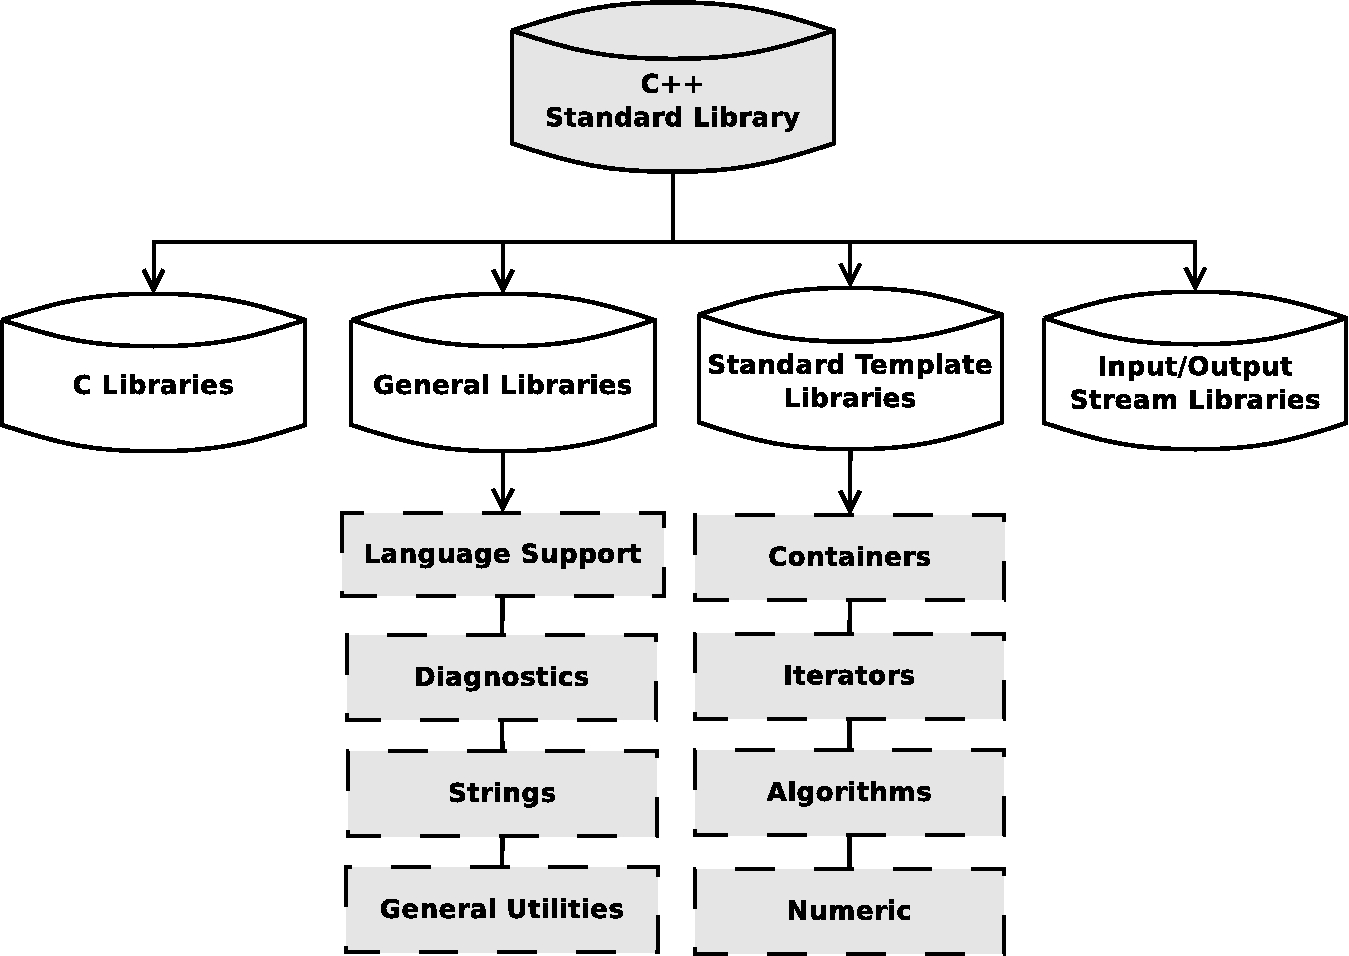
\includegraphics[scale=0.25]{figures/diagramascpp}
\caption{Overview of the operational model.}
\label{figure:cpp-diagram}
\end{figure}

%------------------------------
%\subsection{C Libraries}
%------------------------------

Note that the COM also includes the ANSI-C libraries already
supported by ESBMC.  Since ESBMC++ uses a different front-end, we have to build
a representation of the ANSI-C libraries into the COM; otherwise, ESBMC++ would
not recognize the library methods and fail to parse the C++ programs.
%
However, the biggest part of the COM models 
the Standard Template Libraries (STL).
This part is split into
four categories: \textit{algorithms}, \textit{numeric},
\textit{containers}, and \textit{iterators}.
Apart from that categories, the verification of C++ programs with 
templates is essentially split into two steps: template creation 
and template instantiation. To create a template, ESBMC++ finds 
the respective template declaration and creates an internal representation 
of the class or function by flagging the types as generic; no other representation 
is created here since at this step ESBMC++ does not know which types will be 
instantiated. To instantiate a template, ESBMC++ finds a template usage 
with a specified type and creates a new internal representation of the 
class or function with the instantiated type; this new representation 
is not a template anymore. At this point, ESBMC++ keeps track of the 
generic template definition and the respective instantiated class or function.
When a new template is instantiated, ESBMC++ first checks whether it was already 
instantiated to avoid creating an existing representation of a previously 
instantiated template. 

In this paper, we focus on the operational model of the
sequential containers and iterators in the STL,
%its preconditions and simulation features
%(e.g., how we store the elements values of the containers), 
and how they are used to
verify real-world C++ programs.



%-------------------------------------------
\subsection{Core Container Language}
%-------------------------------------------

To formalize the verification of the STL containers,
we define a core container language, and extend the translation
functions $\cal C$ and  $\cal P$ of constraints and properties to this.
We then use this core language to implement the operational model 
of the containers. Figure~\ref{ccl-fig} summarizes the core container 
syntax.

\begin{figure}
\[\begin{array}{r@{\:\:}r@{\:\:}l}
  T   & ::= & 
    t \:|\: \mathit{*It} \:|\: \mathit{*P} 
\\[0.5ex]
   \mathit{It} & ::= & 
     i \:|\: \mathit{It} (+ \:|\: -) \mathit{It}
       \:|\: \mathit{C.begin} \:|\: \mathit{C.end} 
\\  & | & 
     \mathit{C.insert(It, T, N)} \:|\: \mathit{C.insert(It, It, It)}
\\  & | & 
     \mathit{C.erase(It, It, It)} \:|\: \mathit{C.erase(It)} \:|\: \mathit{C.search(It)}
\\[0.5ex]
   P  & ::= & 
     p \:|\: P (+ \:|\: - ) P
       \:|\: \mathit{It.pointer} \:|\: \: \mathit{It.source}
       \:|\: \mathit{C.array}
\\[0.5ex]
  \mathit{Int}  & ::= & 
     n \:|\: \mathit{Int} (+ \:|\: * | \ldots) \mathit{Int}
       \:|\: \mathit{C.size} \: | \: \mathit{C.capacity}
  \end{array}
\]
  \caption{\label{ccl-fig}Core container syntax}
\end{figure}

The container language comprises several syntactic domains, starting with
the base elements $\mathit{T}$, iterators $\mathit{It}$, pointers $\mathit{P}$,
and integer indices $\mathit{Int}$, and of course the (proper)
container expressions $\mathit{C}$. The syntax for $\mathit{T}$
values is the following:

\[\begin{array}{r@{\:\:}c@{\:\:}l}\label{element-semantics}
%\\[-5ex]
\mathit{T}   & ::= & \: \mathit{t} \: | \: \mathit{*It} \: | \: \mathit{*P} \: | \: \mathit{C_n} \:  
\end{array}
\]

\noindent
Here $\mathit{t}$ is a variable of type $\mathit{T}$ and
$\mathit{*It}$ is the value stored in the position pointed
by an iterator $\mathit{It}$. Similarly, $\mathit{*P}$ is the value
stored in the $\mathit{P}$ position of the memory, and $\mathit{C_n}$ is
an element of a container $\mathit{C}$ in the position $\mathit{n}$.
The syntax for iterator expressions is:

\[\begin{array}{r@{\:\:}c@{\:\:}l}\label{iterator-semantics}
%\\[-5ex]
\mathit{It}   & ::= & \: \mathit{i} \: | \: \mathit{It} ( + \: | \: - ) \mathit{It} \: | \: \mathit{C.begin} \: | \: \mathit{C.end} \:  
\end{array}
\]

\noindent
Here $\mathit{i}$ is a variable of type $\mathit{It}$;
$\mathit{begin}$ and $\mathit{end}$ are methods
that return iterators which point to the beginning
and the ending of a container, respectively. We also have
iterator operations that return iterators as well.
For memory address values $P$, the syntax is as follows:

\[\begin{array}{r@{\:\:}c@{\:\:}l}\label{pointer-semantics}
%\\[-5ex]
\mathit{P}  & ::= & \: \mathit{p} \: | \: \mathit{It.pointer} \: | \: \mathit{C.array} \: | \\
            &     & \: \mathit{It.source} \: | \: \mathit{P}  ( \: + \: | \: - \: )  \textit{P} \: \\
\end{array}
\]

\noindent
Here $\mathit{It.pointer}$ is a memory address that stores the element
in the container pointed by the iterator, $\mathit{C.array}$ is another
memory address that stores the beginning of the container array,
$\mathit{It.source}$ is the address that relates the iterator
and the container it points to.
% (which stores the container $array$ value).
% There is also a pointer return from pointer operations.
The containers contain an array of elements $\mathit{T}$ and their
positions in the memory are represented by pointers $\mathit{P}$.
The syntax for the integer expression is defined as follows:

\[\begin{array}{r@{\:\:}c@{\:\:}l}
%\\[-5ex]
\mathit{Int}  & ::= & \: \mathbb{N} \: | \: \mathbb{Z} \: | \: \mathit{C.size} \: | \: \mathit{C.capacity} \: | \\
              &     & \: \mathit{Int} \: ( + \: | \: ? \: | \: * \: | \: ...) \: \mathit{Int}  \: 
\end{array}
\]

\noindent
Here, $\mathbb{N}$ and $\mathbb{Z}$ represent the natural 
and integer numbers, respectively. $\mathit{C.size}$ and $\mathit{C.capacity}$ 
return the actual and maximum size, respectively of the containter $C$.
%an integer value as well as the arithmetics
%operations between integer values.


%-------------------------------------------
\subsection{Operational Container Model}
%-------------------------------------------

%The structure of the STL containers is based on the
%C++ structure itself, which includes classes, operators,
%methods, functions, and intern variables. 
%We thus split it into:
%iterations, capacity, element access, modifiers, and unique
%members. 
As the container structures differ slightly
between each other, some of their methods will vary too,
changing its intern model as well (e.g., a \textit{list}
container does not have a reference operator and its elements
are only reached by iterators).

To simulate the containers appropriately, our model makes
use of three variables: a variable of type $P$ called \emph{array} that points
to the first element of the array, a natural number \emph{size} that stores
the quantity of elements in the container, and a natural value \emph{capacity}
that stores the total capacity of a container (which is valid only for vectors).
Note that, as the elements are added in the container (specifically in vectors)
and the size grows, the capacity is doubled every time
the size reaches the existing capacity value. Similarly, iterators are modeled using
two variables: a variable of type $\mathbb{N}$ called \emph{pos},
which contains the index value pointed by the iterator in the container and a
variable of type $P$ called \emph{source}, which contains the memory address to the first
element $T$ stored in the container. Figure~\ref{figure:stl-iterator} gives
an overview of our operational model for the STL sequantial container.


\begin{figure}[ht] \centering
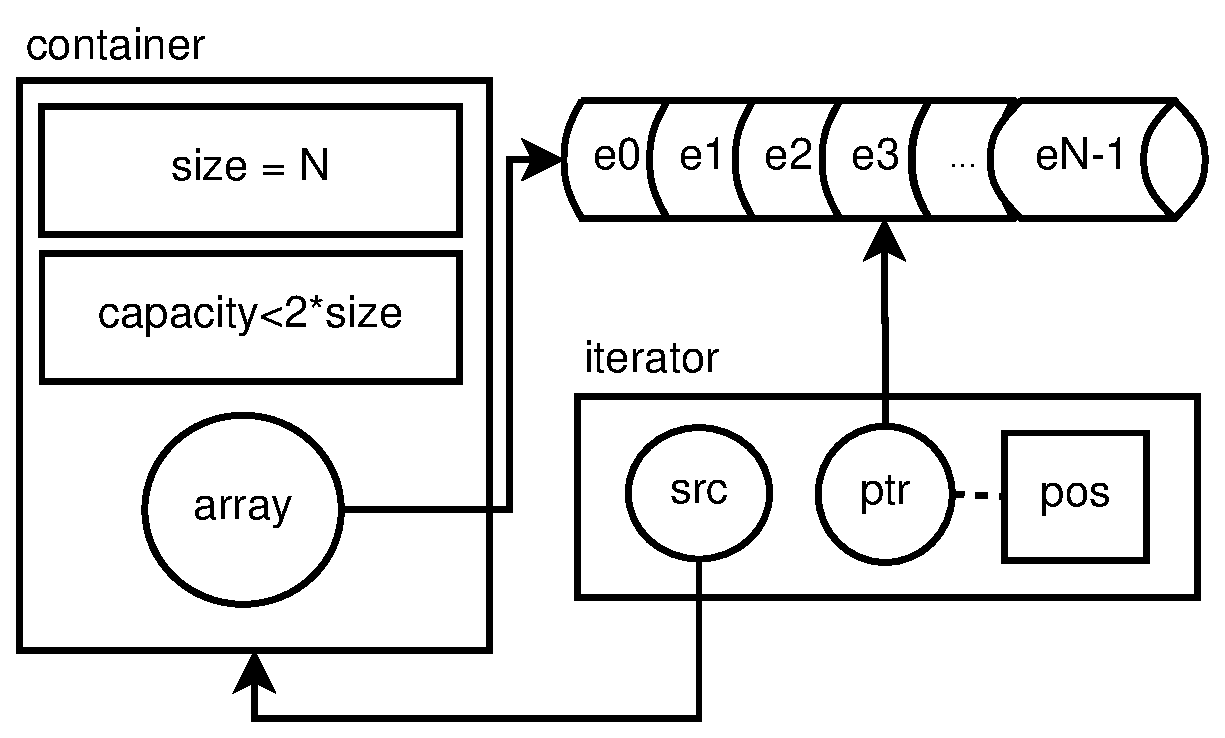
\includegraphics[scale=0.3]{figures/stl-iterator}
\caption{Operational model of the STL sequential container.} 
\label{figure:stl-iterator}
\end{figure}

%The vector container model has the following structure:
%$C = \{ array, size, capacity\}$,
%where $array$ is a memory address where the elements are stored in the container,
%$size$ is the total number of elements in the container, and $capacity$
%is the total capacity of the vector, which is simulated internally in the model.

The main methods of a vector (and the other sequential containers) have only
five types of operation: $\mathit{insert\left(It, T, N\right)}$,
$\mathit{insert\left(It, It, It\right)}$, $\mathit{erase\left(It, It, It\right)}$,
$\mathit{erase\left(It\right)}$, and $\mathit{search\left(It\right)}$.
Methods $push\_back\left(\right)$, $pop\_back\left(\right)$, $front\left(\right)$,
$back\left(\right)$, $push\_front\left(\right)$, and $pop\_front\left(\right)$ are only
a simplified variation of those main methods, which are optimized for some containers
(e.g., popping the last element of a \textit{stack}).
As part of the single static assignment (SSA) transformation, side-effects on the containers 
are made explicit, so that every operation returns a new container as a result. For example,
$\mathit{c.insert\left(x,y,z\right)}$ becomes $\mathit{c' = c.insert\left(x,y,z\right)}$.
The translation function $\cal C$ then describes the constraints relating the ``before''
and ``after'' versions of this structure.

To represent the model, consider a container $C\{\mathit{con}\}$ with a
method $\mathit{con.insert} \rightarrow It$ that returns an iterator result and
makes use of an iterator $It\{ipos\}$ that points to the desired
(insertion) position; a template value $T\{val\}$ with the element
to be inserted and an integer $N\{qtd\}$ that denotes the amount
of elements to be inserted.

\[\begin{array}{ll}
%\label{eqnarray:transformations}
\multicolumn{2}{l}{{\cal C}(con'=con.insert(ipos, val, qtd))=}\\ 
%\Longrightarrow & 
  &  con'.size = con.size + qtd\\
  & \wedge \: *ipos = val \\
  & \ldots \\
  & \wedge \: *(ipos + qtd - 1) = val \\
\end{array}\]

There is another way to represent the insert method.
It is possible to insert a sequence of elements in the desired
insertion position, using both iterator or pointer bounds.
Let $It\{it_0\}$ be an iterator that marks the first element
to be inserted, $It\{it_k\}$ be another iterator that
points to the first element after the end of the sequence to be inserted
in the required position and let $N\{k\}$ be the length of the array $[it_0\, it_k)$.
Thus, we have:

\[\begin{array}{ll}
%\label{eqnarray:transformations}
\multicolumn{2}{l}{{\cal C}(con.insert(ipos, it_0, it_k))=}\\
% \Longrightarrow 
  & con'.size = con.size + k\\
  & \wedge \: *ipos = *it_0 \\
  & \ldots \\
  & \wedge \: *(ipos + k - 1) = *(it_k - 1) \\
\end{array}\]

The same model above is valid for pointers $P\{pt_0\}$ and $P\{pt_k\}$.
This kind of insertion (with pointers) does not return an iterator.

\comment{
In terms of C++ code, we can represent the insertion method as the code:

\begin{figure}[h]
\centering
\begin{minipage}{0.9\textwidth}
\begin{lstlisting}[style=nonumbers]
iterator insert(iterator it, T value){
	assert(size >= 0 && capacity >= size );
	assert(it.ptr != NULL && it.src != NULL);
	int i = size;
	while( i > it.pos - 1){
		array[i+1] = array[i];
		i--;
	}
	array[it.pos] = value;
	size++;
	return it;
}
\end{lstlisting}
\end{minipage}
\caption{Insertion code example}
\label{figure:IR_uml_rec}
\end{figure}

We can also represent the insert method using $C$ and $P$ formulae. The $array$ variable stores the elements of a container, as $size$
indicates the amount of elements stored in a container, and $capacity$ indicates the maximum size a container can reach before
being reallocated in the memory. . The following model
%
\begin{equation}
\label{insertion-formula-c}
C := \left [ \begin{array}{ll}
     array_{n} = store\left(array_{n-1},size_{0} - n - 1 ,select\left(array_{n-1}, size_{0} - n\right)\right) \\
     \wedge array_{n+1} = store\left(array_{n}, size_{0} - n, value\right) \\
              \end{array} \right ],  \\
\end{equation}
\\

\begin{equation}
\label{insertion-formula-P}
P := \left [ \begin{array}{ll}
     \left( size \geq 0 \right) \wedge \left( capacity \geq size \right) \\
     \wedge \left( it.ptr \neq NULL \right) \wedge \left( it.src \neq NULL \right)\\
              \end{array} \right ],  \\
\end{equation}

represents the insertion of a element $value$ in a desired position (in this case, is represented by $size_{0} - 1$).
}


The erase method works similarly to the insert method. It also uses iterator
positions, integer values and pointers, but it does not use values since the exclusion
is made by a given position, regardless the value. It also returns an iterator position,
pointing to the position next to the previously erased part of the container.
The following model shows an \textit{erase} method that deletes a single element:

\[\begin{array}{ll}
%\label{erase1-model}
\multicolumn{2}{l}{{\cal C}(con.erase(ipos)=}\\
% \Longrightarrow 
  & con'.size = con.size - 1 \wedge \: ipos' = ipos + 1 
\end{array}\]

It is also possible to delete a number of elements from the container by
marking the bounds with iterators. It works similarly to the equivalent
\textit{insert} method:

\[\begin{array}{ll}
%\label{erase2-model}
\multicolumn{2}{l}{{\cal C}(con.erase(ipos, it_0, it_k)=}\\
%\Longrightarrow 
  & 	con'.size = con.size - k \wedge \: ipos' = it_k 
\end{array}\]

Searches are made in a container by using reference operators
and a pointing type (pointer or iterator), and return the reference
value (the element stored itself). It can be considered as values
$N\{*It\}$, $N\{*P\}$ or $N\{C_n\}$.	The structure of iterators
is treated differently from other types. The model is the following:
$It = \{n, addr\}$,
where $n$ is the iterator indexed
internally in the container and $addr$ is a memory
address equivalent to $con.array$, where $con$ is the container
pointed by the iterator.

%---------------------------------------------
%\subsection{Input/Output Stream Libraries}
%---------------------------------------------

%%%%%%%%%%%%%%%%%%%%%%%%%%%%%%%%%%%%%%%%%%%%%%%%%%%%%%%%%
%%%%%%%%%%%%%%%%%%%%%%%%%%%%%%%%%%%%%%%%%%%%%%%%%%%%%%%%%
\comment{
To build the operational model, it is important
to define a class structure that is as close as to the
real implementation so that ESBMC++ can correctly identify
the relationships between classes in a given program and
then introduce such relationships to build the AST.}
%%%%%%%%%%%%%%%%%%%%%%%%%%%%%%%%%%%%%%%%%%%%%%%%%%%%%%%%%
%%%%%%%%%%%%%%%%%%%%%%%%%%%%%%%%%%%%%%%%%%%%%%%%%%%%%%%%%

%%%%%%%%%%%%%%%%%%%%%%%%%%%%%%%%%%%%%%%%%%%%%%%%%%%%%%%%%
%%%%%%%%%%%%%%%%%%%%%%%%%%%%%%%%%%%%%%%%%%%%%%%%%%%%%%%%%
\comment{
We have elaborated a hierarchical structure for the
input/output (I/O) stream library that is similar to the actual
one (as described in~\cite{CppReference12}). However,
in our I/O stream operational model, the input operator $>>$
is simply modeled as a non-deterministic variable and we do not check
any related safety property. Similarly, the output operator $<<$ does not
present any constraints or properties to be checked since
we do not check whether a given value has been printed on the screen
(ESBMC++ is only interested in checking the properties related to
software and not that of hardware).}
%%%%%%%%%%%%%%%%%%%%%%%%%%%%%%%%%%%%%%%%%%%%%%%%%%%%%%%%%
%%%%%%%%%%%%%%%%%%%%%%%%%%%%%%%%%%%%%%%%%%%%%%%%%%%%%%%%%


%\begin{figure*}[ht]
%\centering
%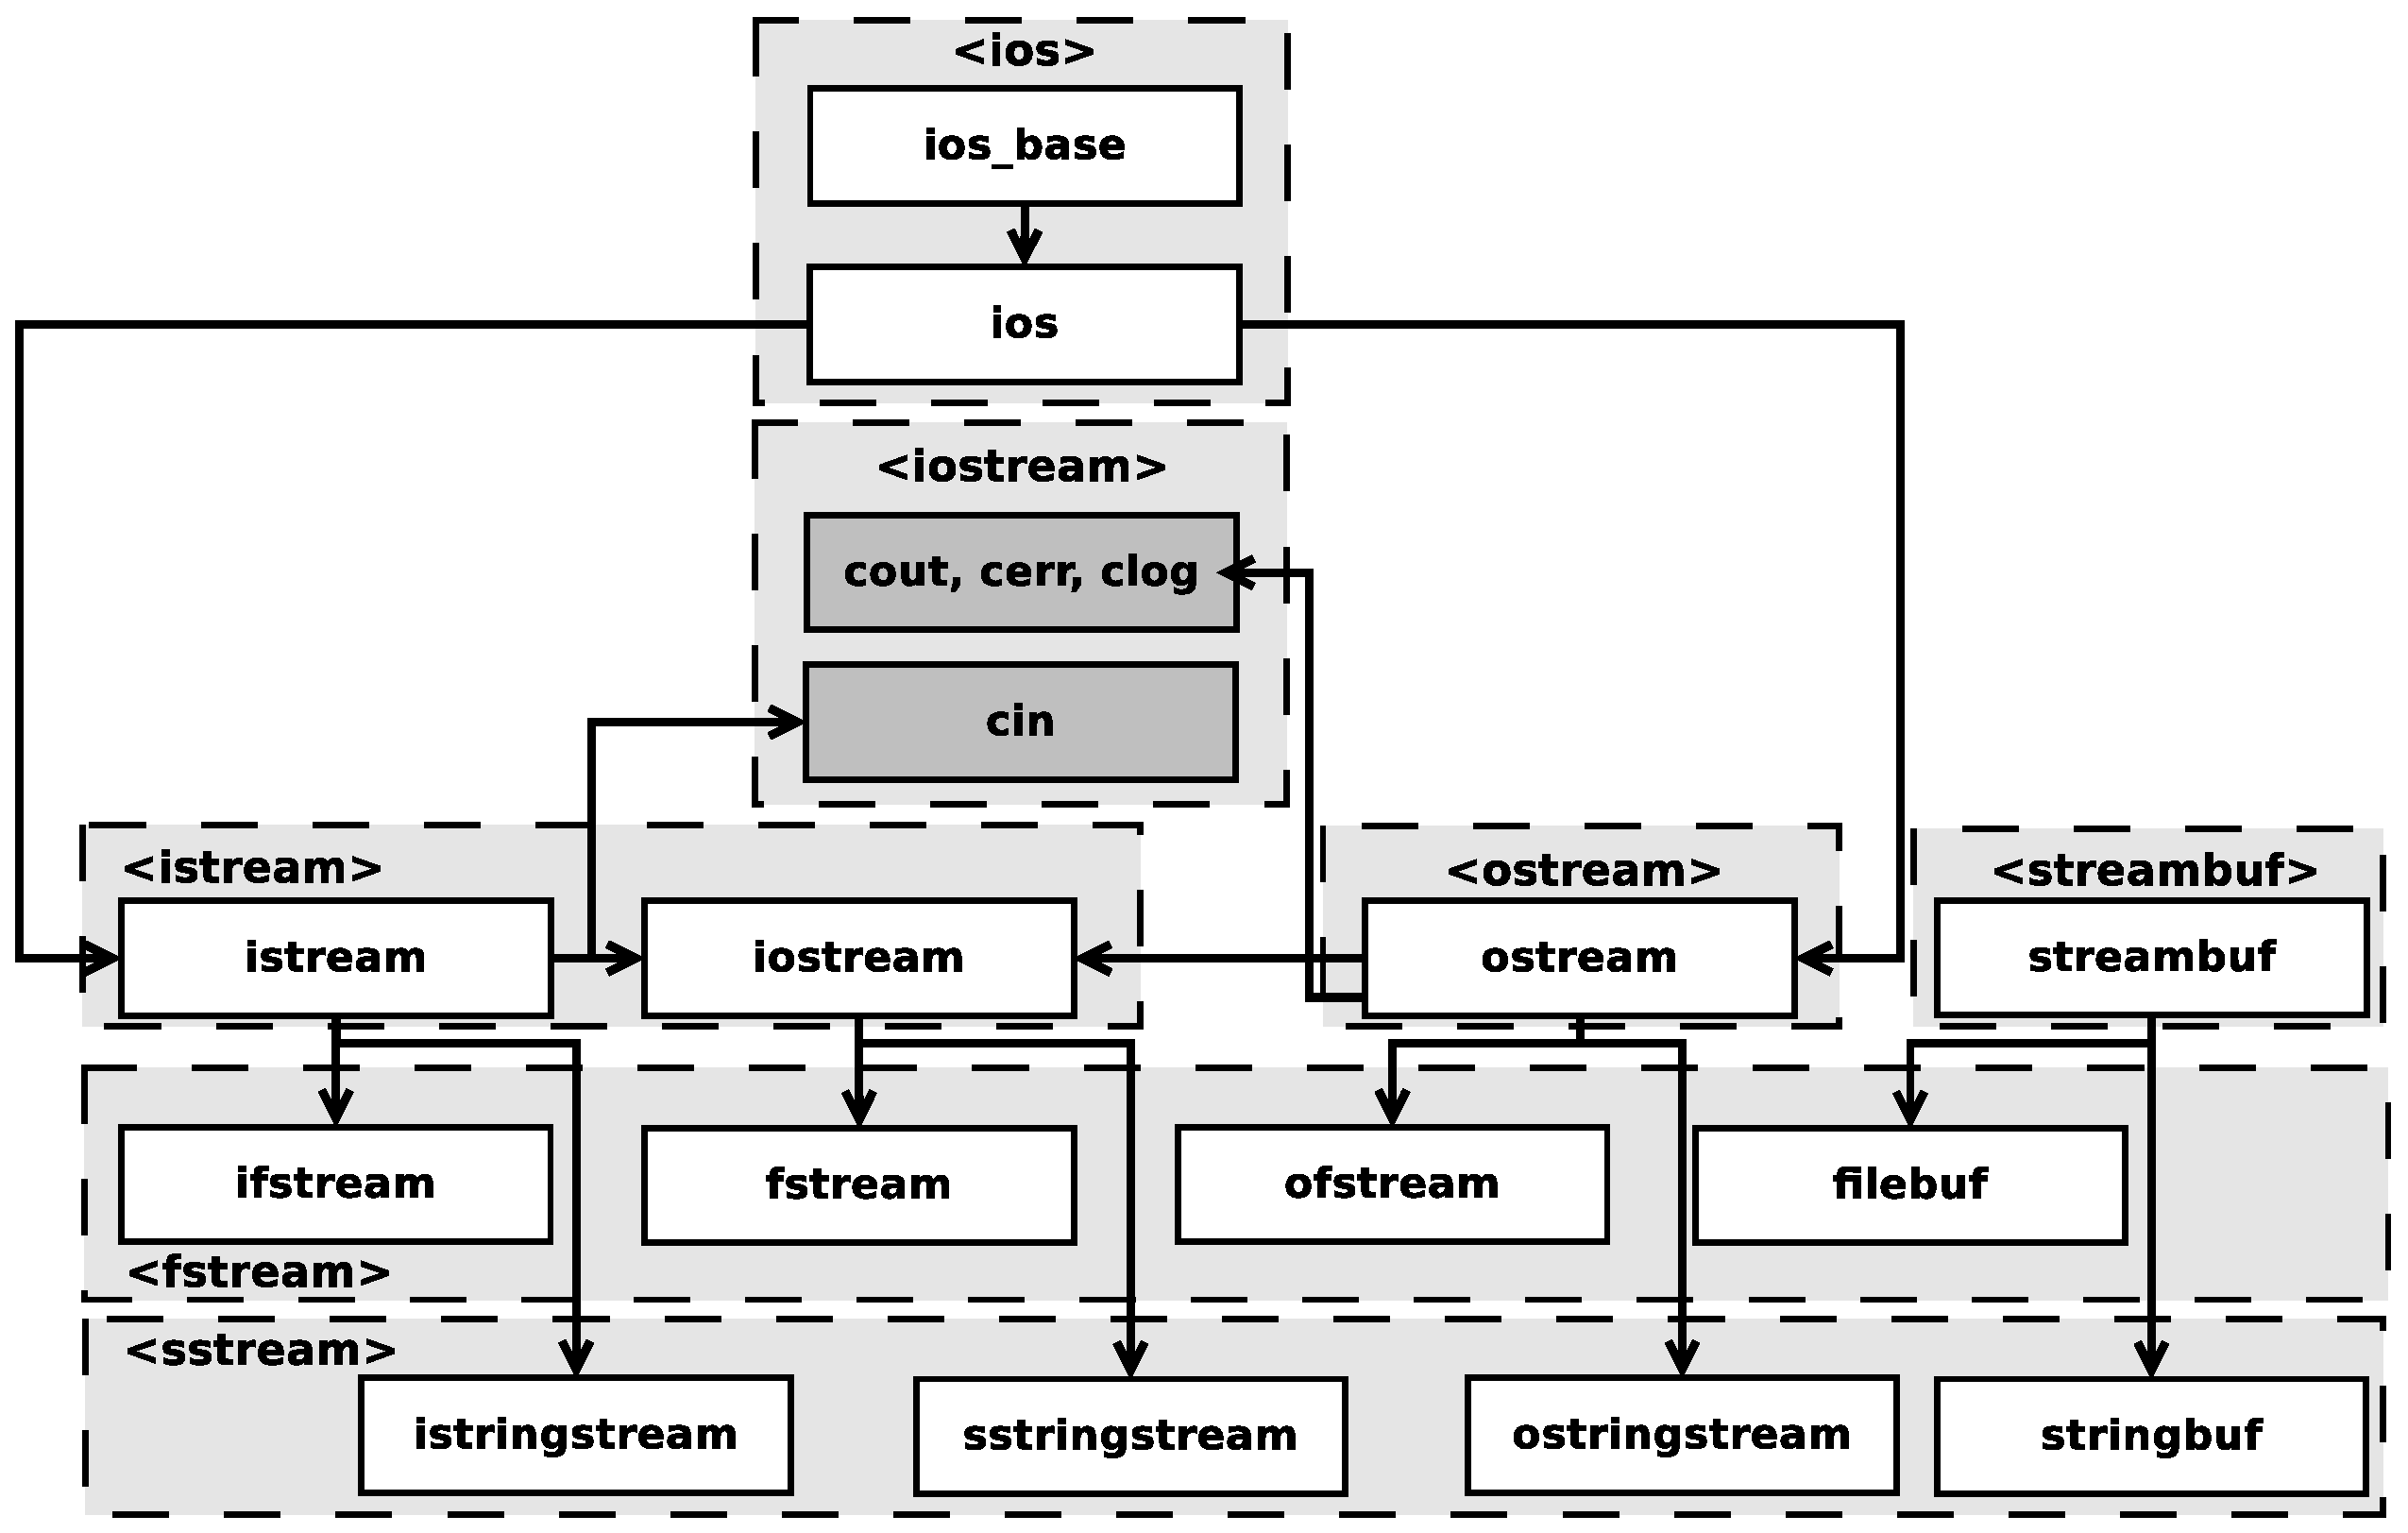
\includegraphics[scale=0.24]{figures/inputoutputdiagram}
%\caption{Hierarchical structure of the Input / Output Stream Libraries.
%Dotted gray square represents the library, white square represents the class and dark gray square represents the access objects.}
%\label{figure:cpp-inputoutputdiagram}
%\end{figure*}


%------------------------------------------------
\section{Inheritance and Polymorphism}
\label{inheritance-and-polymorphism}
%------------------------------------------------

Modeling C++ features like inheritance and polymorphism
makes static analysis difficult to implement.
In contrast to Java, which only allows single inheritance, where derived classes
have only one base class, C++ also allows multiple inheritance, where a class
may inherit from one or more unrelated base classes. This particular feature
makes C++ programs harder to model check than programs in other object-oriented
programming languages (e.g., Java) since it disallows the direct transfer of
techniques developed for other, simpler programming languages.

To deal with inheritance in ESBMC++, we simply replicate the methods
and attributes of the base classes to the inherited class to have
direct access to them. In particular, if a class inherits from
a base class that does not contain virtual methods,
then we call this as \textit{replicated inheritance}. If there is a path from
class $\mathit{X}$ to class $\mathit{Y}$ whose first edge is virtual, then
we call this as \textit{shared inheritance}.

A formal description to represent
the relationship between classes can be described by the class hierarchy graph
(CHG). This graph $\zeta$ is composed of a tuple $\textless \mathit{C}, \prec_{s}, \prec_{r}>$,
where $\mathit{C}$ is the set of classes, $\prec_s $ refers to \textit{shared inheritance} edges,
and $\prec_r$ are \textit{replicated inheritance} edges. The symbols $\prec_{s}$ and $\prec_{r}$
are the set of edges that represent the inheritance relationship between
classes and both sets are in $\mathit{C_{sr}}$ (where $\mathit{C_{sr}} \subseteq \mathit{C} \times \mathit{C}$.
We also consider that $\prec_{sr} = \prec_s \cup \prec_r$ and $\leq_{sr} = (\prec_{sr})^*$.
Additionally, ($\mathit{C}, \leq_{sr}$) are defined as a partially ordered set~\cite{Neggers99}
and $\leq_{sr}$ is anti-symmetric (i.e., if one element A of the set precedes B,
the opposite relation could not exist).

As an example, Figure~\ref{figure:uml_diagram} shows an UML diagram
that represents the \textit{Shape} class hierarchy that contains multiple inheritance.
The Rectangle class relation can be formalized by
($\left(C, \left\langle Rectangle, Shape \right\rangle \right)$,
$\left(C, \left\langle Rectangle, Display \right\rangle \right)$).
Our tool creates an intermediate model for single and multiple inheritance, handling
replicated and shared inheritance where all classes are converted into structures and all
methods and attributes of its parent classes are joined. On the one hand, this approach has
the advantage of having direct access to the attributes and methods
of the derived class and thus allows an easier validation, as the tool
does not search for attributes or methods from base classes on each access.
On the other hand, we replicate information to any new class, thus wasting
memory resources.


\begin{figure}[ht]
\centering
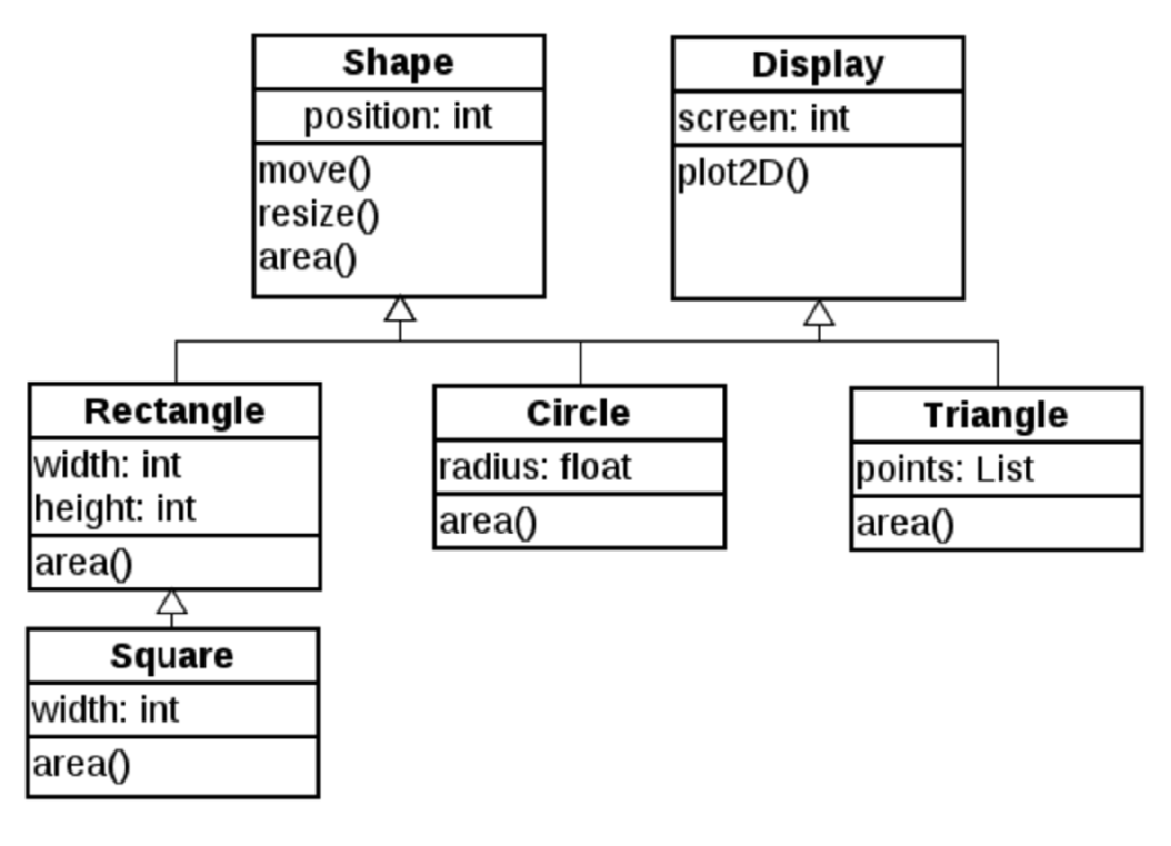
\includegraphics[scale=0.28]{figures/inheritance_uml}
\caption{\textit{Shape} class hierarchy UML diagram} 
\label{figure:uml_diagram}
\end{figure}

Another important feature from object-oriented programming that we
support is the concept of polymorphism, which allows the creation of
reusable code by changing only specific features from the base class.
In this sense, polymorphism allows variable instances to be
bounded to references of different types according to the structure of the
inheritance hierarchy~\cite{Alexander02}.
We thus consider that two or more derived classes
from the same base class can invoke methods with the same signature but 
with distinct behaviors, specialized for each derived class, using for 
this one reference to each object of this base class type. The decision 
of which method must be used cannot be made at compile-time. 
One solution is the usage of virtual tables (described below) that contains 
the object's method address. In this case, the method call will fetch the correct method 
address from this object's dispatch table at verification-time.

%The decision of which method must be used, according to the type
%of the derived class, is chosen in run-time using the late binding of ESBMC++.


The intermediate representation of C++ programs in ESBMC++ provides a model
to handle polymorphism so that we can simplify the class hierarchy,
thus easing the access to methods with the same name without ambiguity between
base and derived classes. As an example, our tool can easily handle the polymorphic
area method using this representation, as shown in Formulas (\ref{area-class-c}) and
(\ref{area-class-p}), using the background theories.
%
\begin{equation}
\label{area-class-c}
C := \left [ \begin{array}{ll}
        j_{1} = store\left(j_{0}, vtable, Rectangle\right) \\
        \wedge j_{2} = store\left(j_{1}, width, 10\right) \\
        \wedge j_{3} = store\left(j_{2}, height, 10\right) \\
        \wedge j_{4} = store\left(j_{3}, vtable, Square\right) \\
        \wedge j_{5} = store\left(j_{4}, width, 10\right) \\
        \wedge return\_value_{1} = \\
        \left(select\left(j_{5}, width\right) \times select\left(j_{5}, width\right)\right) \\
              \end{array} \right ],  \\
\end{equation}
%
\begin{equation}
\label{area-class-p}
P := \left [ \begin{array}{ll}
              return\_value_{1} = 100 \\
              \end{array} \right ]  \\
\end{equation}
%

The classes \textit{Rectangle} (which is the base class)
and \textit{Square} (which is the derived class) have a virtual method
called $area\left(\right)$, which have the same signature. As our running example
calls this method on a base class pointer, then this called function
cannot be determined at compile-time. To overcome this problem,
we thus create a \textit{vtable} to contain the address of the object's bound
methods so that the call to this method is fetched with the address from
the \textit{vtable} at verification-time.

In addition to that, we also support the indirect inheritance,
which is a class that inherits features from a derived class with one
or more classes not directly connected. In Figure~\ref{figure:uml_diagram}, we have
$\left(C, \left\langle Square, Rectangle, Shape \right\rangle \right)$.
Thus, \textit{Square} class can access features from \textit{Shape} class,
but they are not directly connected. We tackle this problem by
looking for the features using a depth search from the derived to base classes
and adding them to our intermediate representation if necessary.

In OO programming, the use of \textit{shared inheritance} is very common.
In contrast to other approaches (e.g.,~\cite{Blanc07}), ESBMC++ is able to
verify this kind of inheritance. If a class has pure virtual methods only,
then this class does not contain any implementation for these methods and they will
thus be implemented in the derived classes. Otherwise, if a class has only virtual
methods, it must contain an implementation for them or the verification will fail
with a ``conversion error''. ESBMC++ also handles virtual destructors successfully
and supports the default constructor creation. Currently, ESBMC++
supports dynamic cast between primitive types, same classes and from a derived
class to a base. ESBMC++ also handles with cast to a reference type, verifying the
correct use of \textit{bad\_cast} thrown by dynamic cast.


%--------------------------------------------
\section{Exception Handling}
\label{exception-handling}
%--------------------------------------------

One of the features that C++ provides is exception handling. 
Exceptions are unexpected situations 
that the program was not designed to handle. The exception handling 
is split into three elements: a try block, where an exception may occur; 
a catch block (also called handler), where an exception can be handled; and a throw 
expression to connect both blocks. Figure~\ref{figure:try-catch-example} 
shows a C++ code example with exception handling.
%
\begin{figure}[ht]
\centering
\begin{minipage}{0.45\textwidth}
\begin{lstlisting}
int main() {
  // try block
  try { 
    throw 20; // throw expression
  } 
  // catch block
  catch (int i) { 
  /*error handling for int exceptions*/ 
  }
  catch (float f) { 
  /*error handling for float exceptions*/ 
  }
  return 0;
}
\end{lstlisting}
\end{minipage}
\caption{Try-catch example: Throwing an integer exception.} 
\label{figure:try-catch-example}
\end{figure}

In ESBMC++, the exception handling happens in two steps:
during the type-checking and the symbolic execution phases.
On the type-checking phase, an AST is built based on the code
inside the try block, but with a few adaptations: before the try block, 
a CATCH instruction with an empty map (which will be filled later on 
the type-checking) is inserted, followed by the respective code inside 
the try block. Here, another CATCH instruction (to represent the end of the 
try block and the beginning of the catch block) is inserted together with 
a GOTO instruction, which aims to point to the code after the catch block. 
This GOTO instruction will only be modified if an exception is thrown;
otherwise it will remain the same. After type-checking the try block,
ESBMC++ type-checks the catch block, which might contain one or more catch blocks.
Again, the AST will be created based on the code inside the catch blocks, but
with only one adaptation: a GOTO instruction is inserted at the end of
each catch block, which aims to point to the code after the catch blocks. Each catch block
will thus be assigned a label so that ESBMC++ can decide which catch should be called
during the symbolic execution phase if an exception is thrown. At the end
of the catch block, the map of the first CATCH instruction is
inserted before the try block code is filled with the label created
for each catch mapped on the type of the exception. Figure~\ref{figure:try-catch-goto}
shows the internal flow of ESBMC++ for the exception handling of the code shown in
Figure~\ref{figure:try-catch-example}.

\begin{figure}[ht]
\centering
\begin{minipage}{0.45\textwidth}
\begin{lstlisting}
...
CATCH signed_int->1, float->2
THROW 20
$TARGET = 3;
if(THROW_TYPE == signed_int)
  $TARGET = 1
else if(THROW_TYPE == float)
  $TARGET = 2
CATCH
GOTO $TARGET
1: int i; 
   /*error handling for int exceptions*/
   GOTO 3
2: float f;
   /*error handling for float exceptions*/ 
3: return 0;
\end{lstlisting}
\end{minipage}
\caption{Try-catch conversion to goto functions.}
\label{figure:try-catch-goto} 
\end{figure}

During the symbolic execution phase, when the first
CATCH instruction is found, the catch map is stacked
for later usage. The idea behind the use of a stack is
that we may have try-catch blocks inside other
try-catch blocks and ESBMC++ should always handle
the most internal first. Following the symbolic execution
for the code that is inside the try block, ESBMC++ will continue 
to execute the code until it finds a throw expression. 
When it happens, ESBMC++ looks at the map for a valid catch 
for the exception thrown; if it finds a valid catch, then the label 
will now be saved, but it will only be handled later;
if it is unable to find an exception, then an error will be thrown.
ESBMC++ will also ignore any other \textit{throw} or \textit{goto} 
instruction after the first \textit{throw} is found, but it will continue 
to verify all the try block code. When the second CATCH is found, 
which means that the try block ended, the catch map is unstacked for
 memory efficiency and the GOTO instruction is thus updated (if needed).

%------------------------------------------------------
\subsection{Throwing and Catching an Exception}
%------------------------------------------------------

A C++ code can throw an exception in several situations other
than explicit throw exception: (a) the operator \textit{new} can throw 
a \textit{bad\_alloc} exception; (b) the operator 
\textit{dynamic$\_$cast} can throw a \textit{bad\_catch}
exception; and (c) the function \textit{typeid} can throw a 
\textit{bad\_typeid} exception.
%Those exceptions are built-in on C++ and are supposed to be 
%handled by the program. 
In the C++ standard~\cite{CppDraft}, 
several rules are defined of how an exception
thrown is connected to a catch block. 
In summary, every time when an exception is thrown and
one of the following rules is {true}, the code jumps 
from the throw expression to the catch block as follows:

\begin{enumerate}
 \item The handler that catchs the exception is the first catch with a matching type: We maintain a list with the order of
       catchs and get the catch with the lower value.
 \item A handler will catch an exception thrown if the type thrown and the type of the handler are the same (ignoring const-volatile
       qualifiers): Here, we simply look for the type of the exception in the catch map and then update the GOTO instruction accordingly 
       if we find a match or we simply return an error, otherwise.
 \item Throwing exceptions of types 
  ``arrays of type T'' and ``functions returning type T'' will be caught by handlers with ``pointer to type T'' and
       ``pointer to function returning type T'' types: Here, the conversion is made on the type-checking and the throw expression 
       throws two exceptions: ``array of type T'' and ``pointer of type T'', and ``function returning type T'' and ``pointer to function 
       returning type T'', respectively. The handler that catchs the exception thrown is defined by the first rule in cases of 
       multiple  matches.
 \item The handler will catch an exception of type T if the handler type is an unambiguous public base class of T: The conversion is 
       similar to the previous rule, but here several exceptions may be thrown: the type of the object and the 
       type of its bases. Again, the handler will be defined by the first rule in cases of multiple matches.
 \item The handler will catch an exception of type pointer T if T's type can be converted to the type of the handler, either by
       qualification conversion or standard pointer conversion: Similar to the previous rules, on the type-checking phase the possible
       conversions based on the catchs types will be thrown with the original pointer type, with the handler being defined by the first 
       rule in cases of multiple matches.
 \item If the exception throw is a pointer, then a handler with type \textit{void*} or \textit{nullptr\_t} can catch it: during the 
       symbolic execution, if no match is found on the map and the exception thrown is a pointer, we simply look for a 
       \textit{void*} or \textit{nullptr\_t} catch and then update the GOTO instruction. If the pointer had a match, then this rules is 
       ignored.
 \item A handler of type ellipsis (...) will catch any thrown exception, and shall be the last handler on the catch block: Similar to the
       last rule, but here it works for every type, if no match is found, ESBMC++ looks for a handler of type ellipsis and update the GOTO
       instruction accordingly if one exists.
 \item If the throw has no arguments, then it should rethrow the last thrown exception: we always keep a reference of the last 
       thrown exception and then update a rethrow if this reference is not \verb|NULL|.
\end{enumerate}

%%%%%%%%%%%%%%%%%%%%%%%%%%%%%%%%%%%%%%%%%%
%%%%%%%%%%%%%%%%%%%%%%%%%%%%%%%%%%%%%%%%%%
\comment{
%--------------------------------------------
\section{Exception Handling}
\label{exception-handling}
%--------------------------------------------

One of the features that C++ provides is the exception handling.
The exceptions are unexpected situations about the program; situations
that the program was not designed to handle. Basically, the exception handling
is divided into three elements: a try block, where an
exception may occur; a catch block, where an exception can be handled; 
and a throw expression to connect both blocks. Figure~\ref{figure:try-catch-example} 
shows a C++ program with exception handling.
%
\begin{figure}[ht]
\centering
\begin{minipage}{1.0\textwidth}
\begin{lstlisting}
int main() {
  try { // try block
    throw 20; // throw expression
  }
  // catch block
  catch (int i) { /* error handling for integer exceptions */ }
  catch (float f) { /* error handling for float exceptions */ }
  return 0;
}
\end{lstlisting}
\end{minipage}
\caption{Try-catch example: Throwing an integer exception.}
\label{figure:try-catch-example}
\end{figure}

In ESBMC++, the exception handling happens in two steps:
during the typechecking phase and the symbolic execution phase.
On the typechecking phase, an AST is built based on the code
inside the try block, with a few adaptations: before the code
inside the try block starts, a CATCH instruction with an empty map
(which will be filled later on the typechecking) is inserted, followed by
the code inside the try block, another CATCH instruction
(to represent the end of the try block and the beginning of the
catch block) and a GOTO instruction pointing to the code after
the catch block. This GOTO will only change if an exception is thrown,
otherwise it will remain the same. After typechecking the try block,
ESBMC++ typechecks the catch block that will contain one or more catchs.
Again, the AST will be created based on the code inside the catchs
with only one adaptation: a GOTO instruction is inserted by the end of
each catch code pointing to the code after the catchs. Each catch code
will be assigned a label so that ESBMC++ can decide which catch should be called
during the symbolic execution phase if an exception is thrown. By the end
of the catch block, the map of the first CATCH instruction is
inserted before the try block code is filled with the label created
for each catch mapped on the type of the exception. Figure~\ref{figure:try-catch-goto}
shows the internal flow on ESBMC++ for exception handling of the code from
Figure~\ref{figure:try-catch-example}.

\begin{figure}[ht]
\centering
\begin{minipage}{1.0\textwidth}
\begin{lstlisting}
main() (c::main):
   CATCH signed_int->1, float->2
   THROW 20
   $TARGET = 3;
   if(THROW_TYPE == signed_int)
     $TARGET = 1
   else if(THROW_TYPE == float)
     $TARGET = 2
   CATCH
   GOTO $TARGET
1: int i;
   /* error handling for integer exceptions */
   GOTO 3
2: float f;
   /* error handling for float exceptions */
3: return 0;
END_FUNCTION
\end{lstlisting}
\end{minipage}
\caption{Try-catch conversion to goto functions.}
\label{figure:try-catch-goto}
\end{figure}

During the symbolic execution phase, when the first
CATCH instruction is found, the catch map is stacked
for later usage. The idea behind the use of a stack is
that we may have try-catch blocks inside other
try-catchs block and ESBMC++ should always handle
the most internal first. Following the symbolic execution
for the code that was inside the try block, ESBMC++ will continue
until it finds a throw expression. When this happens, ESBMC++ will
look at the map for a valid catch for the exception thrown; if it finds
a valid catch, then the label will be saved for now and handled later;
if it was unable to find an exception, then an error will be thrown.
ESBMC++ will also ignore any other throw or goto instruction after
the first throw is found but will continue to verify all the try
block code. When the second CATCH is found, which means that the try
block ended, the catch map is unstacked for memory efficiency
and the GOTO instruction is updated (if needed).

%------------------------------------------------------
\subsection{Exception Handling Language}
%------------------------------------------------------

In order to formalize the verification of exception handling, we
define a exception handling language, which we use to implement
the exception handling verification in C++ programs.

The exception handling language comprises several syntactic domains,
starting with the base elements $\mathit{T}$ and pointers $\mathit{P}$.
The syntax for $\mathit{T}$ values is the following:
%
\[\begin{array}{r@{\:\:}c@{\:\:}l}\label{element-semantics}
\\[-5ex]
\mathit{T}   & ::= & \: \mathit{t_T} \: | \: cvr \: \mathit{t_T} \: | \: \mathit{*P} \: \\
\end{array}
\]
%
Where $\mathit{t_T}$ is a variable of type $\mathit{T}$, $cvr$ is a $const$,
$volatile$ or $restrict$ variable of type $\mathit{T}$ and $\mathit{*P}$
is the value stored in the $\mathit{P}$ position of the memory.
For $\mathit{P}$ (memory address values), the syntax is as follows:
%
\[\begin{array}{r@{\:\:}c@{\:\:}l}\label{pointer-semantics}
\\[-5ex]
\mathit{P}  & ::= & \: \mathit{p} \: | \: \mathit{P_{array}} \: \\
\end{array}
\]
%
where $\mathit{P_{array}}$ is a memory address that stores the beginning
of an array.

%------------------------------------------------------
\subsection{Throwing and Catching an Exception}
%------------------------------------------------------

A C++ code can throw an exception in several situations other
than explicit throw exception: (a) the new operator can throw
a \textit{bad\_alloc} exception, (b) the operator
\textit{dynamic$\_$cast} can throw a \textit{bad\_catch}
exception, and (c) the \textit{typeid} funtion can throw a
\textit{bad\_typeid} exception.
Those exceptions are built-in on C++ and are supposed to be
handled by the program. In the C++ draft standard~\cite{CppDraft}
several rules are defined of how an exception
thrown is connected to a catch (called handlers).

To model the behavior of exception handling in ESBMC++, we define a function
$match \rightarrow T_t$ that returns the handle that matched the thrown type
and makes use of the set of thrown types and the set of handles types.

\[\begin{array}{ll}
match(T_{t1}, T_{t2}, \ldots, T_{tN}, T_{c1}, T_{c2}, \ldots, T_{cN}) \Longrightarrow & rule_1(T_{t1},T_{c1}, T_{c2}, \ldots, T_{cN}) \\
  & \vee \: rule_2(T_{t1},T_{c1}, T_{c2}, \ldots, T_{cN}) \\
  & \ldots \\
  & \vee \: rule_9(T_{t1},T_{c1}, T_{c2}, \ldots, T_{cN}) \\
  & \ldots \\
  & \vee \: rule_1(T_{t2},T_{c1}, T_{c2}, \ldots, T_{cN}) \\
  & \ldots \\
  & \vee \: rule_9(T_{t2},T_{c1}, T_{c2}, \ldots, T_{cN}) \\
  & \ldots \\
  & \vee \: rule_1(T_{tN},T_{c1}, T_{c2}, \ldots, T_{cN}) \\
  & \ldots \\
  & \vee \: rule_9(T_{tN},T_{c1}, T_{c2}, \ldots, T_{cN}) \\
\end{array}\]

The function $match$ itself is composed by several functions called $rule$,
each function $rule$ returns either the handle, if the rule is true, or nil
if the rule is false and makes use of the throw type and the set of handles.
When one of the rules is true, the following rules are ignored.

The functions $rule_1$ and $rule_2$ define a match if $T_{t}$ is equal to $T_{C}$ (ignoring
const-volatile-restrict qualifiers).

\[\begin{array}{ll}
rule_1(T_{t1},T_{c1}, T_{c2}, \ldots, T_{cN}) \Longrightarrow
  (T_{t} = T_{C})\rightarrow select(T_{C}) \\
\end{array}\]

\[\begin{array}{ll}
rule_2(T_{t1},T_{c1}, T_{c2}, \ldots, T_{cN}) \Longrightarrow
  (T_{t} = cvr \: T \: \wedge \: T_{C} = T)\rightarrow select(T_{C})
\end{array}\]

To implement this rule ESBMC++ simply looks for the type of the exception
in the catch map and update the GOTO instruction if it finds a match or
returns an error otherwise).

The third and fourth rules define that throwing ''arrays of type T'' and
''functions returning type T'' with be caught by handlers with
''pointer to type T'' and ''pointer to function returning type T'' types.

\[\begin{array}{ll}
rule_3(T_{t1},T_{c1}, T_{c2}, \ldots, T_{cN}) \Longrightarrow
  (T_{t} = T_{f()} \: \wedge \: T_{C} = T_{f()})\rightarrow select(T_{C}) \\
\end{array}\]

\[\begin{array}{ll}
rule_4(T_{t1},T_{c1}, T_{c2}, \ldots, T_{cN}) \Longrightarrow
  (T_{t} = T[] \: \wedge \: T_{C} = T*)\rightarrow select(T_{C}) \\
\end{array}\]

In ESBMC++ the conversion is made on the type-checking phase and the throw
expression throws two exceptions: ''array of type T'' and ''pointer of type
T'', and ''function returning type T'' and ''pointer to function returning
type T'', respectively.

The fifth rule defines that the handler will catch an exception of type T
if the handler type is an unambiguous public base class of T.
For that we define the binary function $base(T_{2}, T_{1})$, that returns
true if $T_{2}$ is base of $T_{1}$ and returns false, otherwise.

\[\begin{array}{ll}
rule_5(T_{t1},T_{c1}, T_{c2}, \ldots, T_{cN}) \Longrightarrow
  (T_{t} = T_{1} \: \wedge \: T_{C} = T_{2} \: \wedge \: base(T_{2}, T_{1}))\rightarrow select(T_{C}) \\
\end{array}\]

In ESBMC++ the conversion is similar to the conversion of the last rule
but in this case several exception may be thrown: the type of the object
and the type of it's bases.

The sixth rule defines that a handler will catch an exception of type
pointer T if T's type can be converted to the type of the handler, either by
qualification conversion or standard pointer conversion.
For that we define the binary function $implicit\_conv(T_{1}, T_{2})$, that
returns true if $T_{1}$ can be implicit converted to $T_{2}$ and returns false,
otherwise.

\[\begin{array}{ll}
rule_6(T_{t1},T_{c1}, T_{c2}, \ldots, T_{cN}) \Longrightarrow
  (T_{t} = T_{1}* \: \wedge \: T_{C} = T_{2}* \: \wedge \: implicit\_conv(T_{1}, T_{2}))\rightarrow select(T_{C}) \\
\end{array}\]

Again, during the type-checking phase in ESBMC++, the possible conversions based
on the handlers types will be thrown with the original pointer type.

The seventh rule defines that if the exception throw is a pointer then
a handler with type \textit{void*} can also catch it.

\[\begin{array}{ll}
rule_7(T_{t1},T_{c1}, T_{c2}, \ldots, T_{cN}) \Longrightarrow
  (T_{t} = T* \: \wedge \: T_{C} = VOID*)\rightarrow select(T_{C})
\end{array}\]

In ESBMC++, during the symbolic execution phase, if no match is found on the map
and the exception thrown is a pointer, we look for a \textit{void*} catch and update
the GOTO instruction. If the pointer had a match this rules is ignored.

The eighth rule defines that A handler of type ellipsis (...) will catch
any thrown exception, and shall be the last handler on the catch block.

\[\begin{array}{ll}
rule_8(T_{t1},T_{c1}, T_{c2}, \ldots, T_{cN}) \Longrightarrow
  (T_{t} = T \: \wedge \: T_{C} = T_{ellipsis})\rightarrow select(T_{C})
\end{array}\]

In ESBMC++, is similar last rule but works for every type,
if no match is found, ESBMC++ looks for a handler of type ellipsis and
update the GOTO instruction if one exists.

The last rule defines that If the throw has no arguments then it should
re-throw the last thrown exception.

\[\begin{array}{ll}
rule_9(T_{t1},T_{c1}, T_{c2}, \ldots, T_{cN}) \Longrightarrow
  (T_{t} = NULL \: \wedge \: T_{t-1} = T)\rightarrow MATCH(T,T_{C1}, T_{C2}... , T_{CN})
\end{array}\]

ESBMC++ always keeps a reference of the last thrown exception and
updates a rethrow if this reference is not \verb|NULL|.}

%%%%%%%%%%%%%%%%%%%%%%%%%%%%%%%%%%%%%%%%%%
%%%%%%%%%%%%%%%%%%%%%%%%%%%%%%%%%%%%%%%%%%


%------------------------------------------------------
\subsection{Exception Specification}
%------------------------------------------------------

The exception specifications define which exceptions a
function or method (including constructors
and destructors) can throw. Alongside a method or
function declaration a throw expression containing
the exceptions list can define none or
multiple exceptions, which will forbid that
any exception that is not in the exception
specification to go out the function or method. Note
that an exception can still be handled inside
a try-catch block inside the function or method
even if it is not in the exception specification.

The exception specification is handled inside ESBMC++
by inserting a THROW\_DECL instruction after the declaration
of each function or method. In the symbolic execution phase,
the exception specification is stacked and removed in the
END\_FUNCTION instruction by the end of every
function or method. The idea for stacking the exception
specification is the same for catch maps, ESBMC++ may
find function calls to other
function and they may also have their own exception specifications.
Finally, when an exception is thrown, ESBMC++ checks if there is an
exception specification currently valid and if the exception thrown
is allowed to be thrown outside the function. If it is allowed, the
exception handling follows and try to look for an match on the catch
map or will return an error, otherwise.


%-----------------------------------
\section{Experimental Results}
\label{experimental-results}
%-----------------------------------

This section is split into three parts.
The setup is described in Section~\ref{experimental-setup}
while Section~\ref{comparison-to-LLBMC} describes a comparison
between ESBMC++~\cite{esbmc12} and
LLBMC (Low-Level Bounded Model Checker)~\cite{llbmc12}
using a set of standard C++ benchmarks. Some details about LLBMC
are also given in Section~\ref{comparison-to-LLBMC}.
In our experiments, we also tried to use the CBMC model checker~\cite{Clarke04},
but since it has failed in most of our benchmarks (as reported previously
by Merz et~al.~\cite{Florian12}), we do not report any results.
In Section~\ref{verifying-the-sniffer-code}, we describe the results of 
verifying a commercial application from the telecommunications domain using ESBMC++.

%-----------------------------------
\subsection{Experimental Setup}
\label{experimental-setup}
%-----------------------------------

The benchmarks that are used in our comparison consist of 1113 C++ programs.
Around 290 programs are extracted from Deitel's textbook~\cite{Deitel},
16 programs are taken from the NEC benchmark suite~\cite{NeclabsBenchmarkExceptions},
16 programs are taken from the LLBMC benchmark suite~\cite{PrabhuMBIG11},
and the others were developed by us to test all the features that the C++ language
provides. The benchmarks are split into eleven modules, as follows:
\textit{algorithm} contains test cases for methods that involve the
algorithm library; \textit{cpp} contains general test cases of the C++
language that involve the general libraries, multi-threading, and templates.
Additionally, it also contains the LLBMC benchmarks and most of the Deitel
benchmarks. The categories \textit{deque}, \textit{list}, \textit{queue},
\textit{stack}, \textit{stream}, \textit{string}, and \textit{vector} contain test cases
for the respective STL container structures.
Finally, \textit{inheritance} contains test cases related to inheritance and
polymorphism while \textit{try\_catch} contains test cases related to exception handling;
the NEC test cases are located in this module.

All the experiments were conducted on an otherwise idle Intel Core i7-2600,
3.40 GHz with 24 GB of RAM running Ubuntu 64-bits. For all the modules,
the individual time limit and memory limit for each test has been set to 900 seconds
and 24 GB (22 GB of RAM and 2 GB of virtual memory), respectively.
The times given were measured using the \textit{time} command.

%-----------------------------------
\subsection{Comparison to LLBMC}
\label{comparison-to-LLBMC}
%-----------------------------------

This subsection describes the evaluation of ESBMC++
against LLBMC, another C++ BMC tool developed by Merz et al.~\cite{Florian12}.
Table~\ref{table:results-of-the-comparison-between-ESBMC-and-LLBMC}
summarizes the results. Here, \textit{N} is the number of C++ programs,
\textit{L} is the total lines of code of each suite, \textit{Time} is the
total verification time of each module, \textit{P} is the
number of correct positive results (i.e., the tool reports SAFE correctly), 
\textit{N} is the number of correct negative results (i.e., the tool reports 
UNSAFE correctly), \textit{FP} is the number of false positive
results (i.e., the tool reports SAFE incorrectly), \textit{FN} is the number
of false negative results (i.e., the tool reports UNSAFE incorrectly), \textit{Fail}
is the number of internal errors during the verification of each module,
\textit{TO} represents the number of time-outs (i.e., the tool was
aborted after 900 seconds),
and \textit{MO} represents the number of memory-outs.

\begin{table*}[t!]
\begin{adjustwidth}{-0.5cm}{}
\renewcommand\arraystretch{1.18}
\setlength{\tabcolsep}{4pt}
\begin{center} {\small
\begin{tabular}{|c|l|r|r||r|r|r|r|r|r|r|r|r|r|r|r|r|r|r|r|}
\hline
  & & & & \multicolumn{8}{c|}{ESBMC++}
        & \multicolumn{8}{c|}{LLBMC} \\  \cline{5-20}
  & Testsuite   & $N$  & $L$   & Time  & P    & N   & FP  & FN   & Fail & TO   & MO    & Time   & P   & N   & FP  & FN  & Fail & TO  & MO \\\hline
1 & Algorithm   & 127  & 3376  & 449   & 61   & 37  & 15  & 14   & 0    & 0    & 0     & 22964  & 53  & 45  & 1   & 2   & 0    & 24  & 2\\ % OK
\hline
2 & Deque       & 43   & 1239  & 221   & 19   & 20  & 0   & 4    & 0    & 0    & 0     & 8585   & 16  & 17  & 0   & 0   & 1    & 9   & 0\\ % OK
\hline
3 & Vector      & 146  & 6853  & 1160  & 99   & 37  & 3   & 7    & 0    & 0    & 0     & 7234   & 91  & 38  & 1   & 3   & 4    & 6   & 3\\ % OK
\hline
4 & List        & 68   & 2292  & 2510  & 24   & 22  & 6   & 14   & 0    & 2    & 0     & 2562   & 5   & 26  & 5   & 28  & 0    & 0   & 4\\ % OK
\hline
5 & Queue       & 14   & 328   & 64    & 7    & 7   & 0   & 0    & 0    & 0    & 0     & 45     & 6   & 7   & 0   & 1   & 0    & 0   & 0\\ % OK
\hline
6 & Stack       & 12   & 286   & 33    & 6    & 6   & 0   & 0    & 0    & 0    & 0     & 45     & 6   & 6   & 0   & 0   & 0    & 0   & 0\\ % OK
\hline
7 & Inheritance & 51   & 3460  & 236   & 29   & 17  & 1   & 2    & 2    & 0    & 0     & 122    & 32  & 12  & 1   & 3   & 3    & 0   & 0\\ % OK
\hline
8 & Try\_catch  & 67   & 4743  & 251   & 15   & 46  & 2   & 3    & 1    & 0    & 0     & 4      & 0   & 1   & 0   & 0   & 66   & 0   & 0 \\ % OK
\hline
9 & Stream      & 66   & 1831  & 1002  & 52   & 13  & 0   & 1    & 0    & 0    & 0     & 11     & 17  & 13  & 0   & 35  & 1    & 0   & 0\\ % OK
\hline
10 & String     & 231  & 4921  & 20555 & 106  & 119 & 5   & 3    & 0    & 0    & 0     & 37     & 6   & 121 & 4   & 102 & 0    & 0   & 0\\ % OK
\hline
11 & Cpp        & 338  & 26624 & 1032  & 267  & 37  & 7   & 24   & 4    & 0    & 0     & 3260   & 235 & 24  & 10  & 52  & 15   & 2   & 1\\ % OK
\hline\hline
  &             & 1165 & 55953 & 27513 & 685  & 361   & 39   & 72  & 7  & 2    & 0     & 44869  & 467 & 310 & 22  & 226 & 90   & 41  & 10\\ % OK
\hline
\end{tabular} }
\end{center}
\caption{Results of the comparison between ESBMC v1.20 and LLBMC v2012.2a.} 
\label{table:results-of-the-comparison-between-ESBMC-and-LLBMC}
\end{adjustwidth}
\end{table*}

The tool developed by Merz et al.~\cite{Florian12} is called LLBMC.
We invoked both tools using two scripts: one for ESBMC++, that reads
the parameters from a file and calls the tool%
\footnote[1]{esbmc -\/-unwind \textit{B}  -\/-no-unwinding-assertions -I /libraries/}
and another for LLBMC, that first compiles the code to bytecode using CLANG~\cite{CLANG},%
\footnote[2]{/usr/bin/clang++ -c -g -emit-llvm *.cpp -fno-exceptions \newline /usr/bin/llvm-link *.o -o main.bc}
reads the parameters from a file and calls the tool.\footnote[3]
{llbmc -\/-ignore-missing-function-bodies \newline -\/-no-max-loop-iterations-checks -\/-max-loop-iterations=\textit{B}}
The bound set for both tools (value of \textit{B}) depends of each test case.
LLBMC currently does not support exception handling and all the bytecodes were generated without
exception support (flag -fno-exceptions) while verifying with LLBMC.
Enabling exceptions resulted in LLBMC aborting in most of the cases.

As we can see in Table~\ref{table:results-of-the-comparison-between-ESBMC-and-LLBMC},
LLBMC times out in 24 programs in the \textit{Algorithm} module and
runs out of memory in two programs. If we carefully analyze those test cases,
most of them use iterators, which might be causing the slow down
in the verification process, which is a situation that also happens in others modules.
In the \textit{Deque}, \textit{Vector}, and \textit{List} modules,
the slowdowns still happen but with small values. The module that had the
most unsuccessful verification results was the \textit{List} module, and most of the
errors were related to the container size (e.g., assertions if the container
is empty or if it has a particular size). In ESBMC++, most of the errors on
those modules are due to a missing operational model
of the libraries, which are currently under development.

In the \textit{Queue} module, LLBMC fails in a program that uses the size of a list
as constructor parameter while in the \textit{Stack} module all programs are correctly verified.
In ESBMC++, all the programs in both modules are successfully verified.

In the \textit{Stream} module, most of the errors are related to assertions on the size
of the stream (using the method $gcount\left(\right)$) and to internal flags (such as
\textit{ios::hex} and \textit{iostream::hex}). In ESBMC++, most of the error are related
to a bad operational model of the internal flags. In the \textit{String} module, the errors are related
to assertions in the string itself, usually if the string is equal to another string.
In the \textit{Inheritance} module, LLBMC reports incorrect errors about memory writing and
instantiation of virtual methods (that do not contain implementation). 
It also does not support some expressions in the SMT back-end (e.g., 
``Op \% (nondef) found''). ESBMC++ fails to verify test cases related to the use of the
\textit{dynamic\_cast} (as described in Section~\ref{inheritance-and-polymorphism}).

In the \textit{try\_catch} module, LLBMC failed in most of the tests due to the fact that
the tool is missing support to exception handling. ESBMC++ was able to verify most of the cases.
The errors that occur are related to a missing implementation of exception specifications when
using classes constructors. And lastly, in the \textit{cpp} module, which has test cases involving all
the other modules (but are not redundant), most of the errors presented were already seen during
the verification of other modules.

ESBMC++ verified all modules in 27513 seconds (approximately 7 hours)
and successfully verified 1046 out of 1165 (89\%) while LLBMC verified all modules
in 44869 seconds (approximately 12 hours) and successfully verified 777 out of 1165
(66\%). We can see that LLBMC is slower than ESBMC++ on the containers
and \textit{algorithm} modules, while it is faster on \textit{stream} and
\textit{string} modules but looses on successfully verified test cases.
In the \textit{Inheritance} module, the results of both tools are essentially the same.
In the \textit{try\_catch} module, ESBMC++ is able to verify almost all programs,
something that LLBMC cannot due to its lack of support of exception handling.
In the \textit{cpp} module, ESBMC++ is able to successfully verify more programs than LLBMC.
Note that ESBMC++ does not crash or runs out of memory or time in any module.

%-----------------------------------
\subsection{Verifying the Sniffer Code}
\label{verifying-the-sniffer-code}
%-----------------------------------

This section describes the results of the verification process using the 
ESBMC++ and LLBMC model checkers against the sniffer code provided by 
Nokia Institute of Technology (INdT). The sniffer code is responsible for 
capturing and logging traffic passing over a network that supports the Message 
Transfer Part Level 3 User Adaptation Layer (M3UA); it enables the transport of 
Signaling System 7 (SS7) protocol’s user parts and it uses the services provided
by the Stream Control Transmission Protocol (SCTP). The sniffer code contains 
approximately 20 classes, 85 methods, and 2839 lines of C++ code. 

The following properties were verified using the customer version 
of the sniffer code: array bounds, division by zero, and arithmetic under- 
and over-flow. Due to confidential issues, we were able to model check 
50 out of 85 methods (since we did not have access to some external classes that 
the sniffer code requires). In this sense, ESBMC++ was able to identify five bugs 
that are mostly related to arithmetic under- and over-flow while LLBMC was able to 
identify only three of them. Note that all bugs were reported to the developers 
and confirmed by them.

As an example of the bugs that were found, Figure~\ref{figure:PacketM3UA} shows 
a code fragment of the method \textit{getPayloadSize} from the class \textit{PacketM3UA}.
Here, an arithmetic over-flow might occur on the typecast operation since the method 
\textit{ntohs} returns an unsigned integer, but the method \textit{getPayloadSize} is
expected to return an integer data-type. One possible way to fix this bug is to change the return type 
of the method \textit{getPayloadSize} to unsigned integer to avoid the typecast over-flow.

\begin{figure}[ht]
\centering
\begin{minipage}{0.45\textwidth}
\begin{lstlisting}
int PacketM3UA::getPayloadSize() {
  return ntohs(m3uaParamHeader->paramSize)
          - (M3UA_PROTOCOL_DATA_HEADER_SIZE 
          + M3UA_PARAMETER_HEADER_SIZE);
}
\end{lstlisting}
\end{minipage}
\caption{Arithmetic over-flow on the typecast operation of the \textit{getPayloadSize}.} 
\label{figure:PacketM3UA}
\end{figure}

%-----------------------------------
\section{Related Work}
\label{related-work}
%-----------------------------------

The application of SMT-based BMC to software is gaining
popularity in the software engineering community mainly due
to the advent of sophisticated SMT solvers built over efficient
SAT solvers~\cite{CVC07,Boolector09,Z08}. 
Previous work related to
SMT-based BMC for software addresses the problem of verifying C programs
that use bit operations, floating-point arithmetic, and
pointers~\cite{Clarke04,Armando09,Ganai06,Cordeiro12}.
However, there is only little work that addresses the problem
of model checking C++ programs that make use of templates, containers,
and exception handling. 

Prabhu et al.~\cite{PrabhuMBIG11} present an interprocedural
exception analysis and transformation framework for C++ that
records the control-flow created by the exceptions
and creates an exception-free program. The exception-free
program creation starts by generating a modular interprocedural
exception control-flow graph (IECFG). The IECFG is refined using
an algorithm based on a compact representation for a set of types
called the Signed-TypeSet domain and the result is used
to generate the exception-free program. Finally, the exception-free
program is verified using F-SOFT~\cite{Fsoft}. The verification is
focused on two properties: ``no throw'', the percentage of the code
that does not raise an exception and ``no leak'', the number of memory
leaks on try-catch blocks \cite{PrabhuMBIG11}.

Jing Yang et~al.\ present a translation tool called Class Hierarchy
Representation Object Model Extension (CHROME) that is targeted towards
making static program analyzers for C++ easier to write and provide
more precise results~\cite{Yang12}. CHROME makes a source-to-source transformation
from a C++ program with inheritance into a semantically equivalent program without
inheritance by treating the inheritance as separate memory regions
that are linked to each other via additional base class and derived class
pointer fields. This transformation comprises a clarifier, which makes
implicit C++ features explicit. This approach was also implemented with 
F-SOFT~\cite{Fsoft}. CHROME has a
different memory behavior from the original program and therefore does not allow
the use of low-level primitives (e.g, \textit{memset}). The CHROME-lowered C program is
three to five times bigger than the size of the original C++ program.

Blanc et~al.\ describe the verification of C++ programs (that use the STL containers)
via predicate abstraction~\cite{Blanc07}. They make use of abstract data types for the STL
usage verification rather than the actual STL implementation and behavior.
Blanc et~al.\ show that it suffices to verify correctness using an operational model
by proving that the pre-conditions on operations in the model imply the pre-conditions
guaranteed by the language definition for those operations; similarly, the post-conditions
given by the standard imply the strongest post-conditions for the operational model.
This approach is efficient in finding trivial errors in C++ programs, but it lacks
on a deeper search for bugs and misleading operations (i.e, when it involves internal
modeling of the methods).

Merz et~al.\ describe the LLBMC tool, which also applies BMC to the verification
of C++ programs~\cite{Florian12}. However, they use the LLVM compiler to convert C++
programs into the LLVM's intermediate representation, which thus looses high-level
information about the structure of the C++ programs (i.e., the relationship between
the classes). Similarly to ESBMC++, Merz et~al.\ also apply SMT solvers to check the verification
conditions that are generated from the C++ programs. In contrast to our approach, however,
they do not handle exceptions, which thus make it difficult to verify realistic C++ programs
(e.g., programs that depend on the STL library).

Java PathFinder is an explicit-state model checker for Java programs, but
Pasareanu and Visser~\cite{Pasareanu04} also developed a symbolic execution 
framework for it. However, due to the considerable differences between 
Java and C++ it is difficult to compare this to ESBMC++.


% An example of a floating figure using the graphicx package.
% Note that \label must occur AFTER (or within) \caption.
% For figures, \caption should occur after the \includegraphics.
% Note that IEEEtran v1.7 and later has special internal code that
% is designed to preserve the operation of \label within \caption
% even when the captionsoff option is in effect. However, because
% of issues like this, it may be the safest practice to put all your
% \label just after \caption rather than within \caption{}.
%
% Reminder: the "draftcls" or "draftclsnofoot", not "draft", class
% option should be used if it is desired that the figures are to be
% displayed while in draft mode.
%
%\begin{figure}[!t]
%\centering
%\includegraphics[width=2.5in]{myfigure}
% where an .eps filename suffix will be assumed under latex, 
% and a .pdf suffix will be assumed for pdflatex; or what has been declared
% via \DeclareGraphicsExtensions.
%\caption{Simulation Results}
%\label{fig_sim}
%\end{figure}

% Note that IEEE typically puts floats only at the top, even when this
% results in a large percentage of a column being occupied by floats.


% An example of a double column floating figure using two subfigures.
% (The subfig.sty package must be loaded for this to work.)
% The subfigure \label commands are set within each subfloat command, the
% \label for the overall figure must come after \caption.
% \hfil must be used as a separator to get equal spacing.
% The subfigure.sty package works much the same way, except \subfigure is
% used instead of \subfloat.
%
%\begin{figure*}[!t]
%\centerline{\subfloat[Case I]\includegraphics[width=2.5in]{subfigcase1}%
%\label{fig_first_case}}
%\hfil
%\subfloat[Case II]{\includegraphics[width=2.5in]{subfigcase2}%
%\label{fig_second_case}}}
%\caption{Simulation results}
%\label{fig_sim}
%\end{figure*}
%
% Note that often IEEE papers with subfigures do not employ subfigure
% captions (using the optional argument to \subfloat), but instead will
% reference/describe all of them (a), (b), etc., within the main caption.


% An example of a floating table. Note that, for IEEE style tables, the 
% \caption command should come BEFORE the table. Table text will default to
% \footnotesize as IEEE normally uses this smaller font for tables.
% The \label must come after \caption as always.
%
%\begin{table}[!t]
%% increase table row spacing, adjust to taste
%\renewcommand{\arraystretch}{1.3}
% if using array.sty, it might be a good idea to tweak the value of
% \extrarowheight as needed to properly center the text within the cells
%\caption{An Example of a Table}
%\label{table_example}
%\centering
%% Some packages, such as MDW tools, offer better commands for making tables
%% than the plain LaTeX2e tabular which is used here.
%\begin{tabular}{|c||c|}
%\hline
%One & Two\\
%\hline
%Three & Four\\
%\hline
%\end{tabular}
%\end{table}


% Note that IEEE does not put floats in the very first column - or typically
% anywhere on the first page for that matter. Also, in-text middle ("here")
% positioning is not used. Most IEEE journals/conferences use top floats
% exclusively. Note that, LaTeX2e, unlike IEEE journals/conferences, places
% footnotes above bottom floats. This can be corrected via the \fnbelowfloat
% command of the stfloats package.

%------------------------------------------------------
\section{Conclusions}
\label{conclusions}
%------------------------------------------------------

In this work, we have investigated SMT-based verification of C++ programs
by focusing on the major features that the language offers. We have described
an implementation of an operational model of the sequential STL containers
as well as novel approaches to handle inheritance, polymorphism, and exception handling
(in particular, exception specification, which is a feature that is not supported by others
BMC tools). Our experiments contain C++ programs with most of the features that C++ language 
has to offer. Additionally, we have verified a commercial application (called sniffer code) of medium-size 
used in the telecommunications domain. The results show that ESBMC++ outperforms LLBMC if we 
consider the verification of C++ programs. In particular, ESBMC++ is able to verify most of the 
C++ programs with an advantage: we are able to verify programs
with exceptions enabled (a missing feature of LLBMC that decreases the verification accuracy of
C++ programs). In addition, ESBMC++ was able to find undiscovered bugs in the sniffer code that
were later confirmed by developers. For future work, we intend to extend the operational model of STL containers
to support not only sequential containers, but also mapped ones (e.g., map and multimap).


% conference papers do not normally have an appendix


% use section* for acknowledgement
\section*{Acknowledgment}
The development of ESBMC++ is funded by the Royal Society and by Nokia Institute of Technology (INdT). 

% trigger a \newpage just before the given reference
% number - used to balance the columns on the last page
% adjust value as needed - may need to be readjusted if
% the document is modified later
%\IEEEtriggeratref{8}
% The "triggered" command can be changed if desired:
%\IEEEtriggercmd{\enlargethispage{-5in}}

% references section

% can use a bibliography generated by BibTeX as a .bbl file
% BibTeX documentation can be easily obtained at:
% http://www.ctan.org/tex-archive/biblio/bibtex/contrib/doc/
% The IEEEtran BibTeX style support page is at:
% http://www.michaelshell.org/tex/ieeetran/bibtex/
%\bibliographystyle{IEEEtran}
% argument is your BibTeX string definitions and bibliography database(s)
%\bibliography{IEEEabrv,../bib/paper}
%
% <OR> manually copy in the resultant .bbl file
% set second argument of \begin to the number of references
% (used to reserve space for the reference number labels box)


%\begin{thebibliography}{1}

%\bibitem{IEEEhowto:kopka}
%H.~Kopka and P.~W. Daly, \emph{A Guide to \LaTeX}, 3rd~ed.\hskip 1em plus
%  0.5em minus 0.4em\relax Harlow, England: Addison-Wesley, 1999.

%\end{thebibliography}

%\renewcommand\refname{{\normalsize References}}
\begin{thebibliography}{1}

\bibitem{CppDraft}
Working draft, Standard for Programming Language {C}++, http://www.open-std.org/JTC1/SC22/WG21/docs/papers/2012/n3376.pdf, 2012.

\bibitem{CppReference12}
Reference of the C++ Language Library, http://www.cplusplus.com/reference/, 2012.

\bibitem{esbmc12}
Efficient SMT-Based Context-Bounded Model Checker, http://esbmc.org/, 2012.

\bibitem{llbmc12}
The Low-Level Bounded Model Checker, http://llbmc.org/, 2012.

\bibitem{CLANG}
LLVM Tools, http://llvm.org/releases/, 2012.

\bibitem{NeclabsBenchmarkExceptions}
NEC, http://www.nec-labs.com/research/system/, 2012.

\bibitem{smtlib09}
{SMT}-LIB, http://combination.cs.uiowa.edu/smtlib, 2009.

\bibitem{Alexander02}
R. T.~Alexander, J.~Offutt, and J. M.~Bieman.
\newblock {Fault Detection Capabilities of Coupling-based OO Testing}
\newblock In {\em ISSRE} pp.~207--2002, 2002.

\bibitem{Armando09}
A.~Armando, J.~Mantovani, and L.~Platania.
\newblock Bounded model checking of software using {SMT} solvers instead of
  {SAT} solvers.
\newblock In {\em STTT}, vol. 11 (1), pp. 69--83, 2009.

\bibitem{CVC07}
C.~Barrett and C.~Tinelli, {CVC}3.
\newblock In {\em CAV}, LNCS 4590, pp. 298--302, 2007.

\bibitem{handbook09}
A.~Biere.
\newblock Bounded model checking.
\newblock In {\em Handbook of Satisfiability}, pp. 457--481. 2009.

\bibitem{Blanc07}
N.~Blanc, A.~Groce, and D.~Kroening,
\newblock Verifying C++ with STL containers via predicate abstraction.
\newblock In {\em ASE}, pp. 521--524. 2007.

\bibitem{Bradley07}
A.~R. Bradley and Z.~Manna. {The Calculus of Computation: Decision
  Procedures with Applications to Verification}.\hskip 1em plus 0.5em minus
  0.4em\relax Springer, 2007.

\bibitem{Boolector09}
R.~Brummayer and A.~Biere, Boolector: An efficient {SMT} solver for  bit-vectors and arrays.
\newblock In {\em TACAS}, LNCS 5505, pp. 174--177, 2009.

\bibitem{Cimatti10}
%A.~Cimatti, A.~Micheli, I.~Narasamdya, and M.~Roveri.
A.~Cimatti et~al.
\newblock Verifying {SystemC}: a software model checking approach.
\newblock In {\em FMCAD}, 2010, pp.\ 121--128.

\bibitem{Clarke04}
E.~Clarke, D.~Kroening, and F.~Lerda.
\newblock A tool for checking {ANSI-C} programs.
\newblock In {\em TACAS}, {\em LNCS} 2988, pp.\ 168--176, 2004.

\bibitem{Cordeiro12}
L.~Cordeiro, B.~Fischer, and J.~Marques-Silva.
\newblock {SMT}-based bounded model checking for embedded {ANSI-C} software.
\newblock In {\em IEEE Trans. Software Eng.}, v.\ 38, n.\ 4, pp.\ 957--974, 2012.

\bibitem{Z08}
L.~M. de~Moura and N.~Bj{\o}rner, Z3: An efficient {SMT} solver.
\newblock In {\em  TACAS}, LNCS 4963, pp. 337--340, 2008.

\bibitem{Deitel}
P.~Deitel and H.~Deitel.
\newblock {C++ How to Program}.
\newblock Prentice Hall, 5th Edition, 2006.

\bibitem{Ganai06}
M.~K. Ganai and A.~Gupta.
\newblock Accelerating high-level bounded model checking.
\newblock In {\em ICCAD}, pp. 794--801, 2006.

\bibitem{Fsoft}
%F.~Ivancic, I.~Shlyakhter, A.~Gupta, M.~Ganai, V.~Kahlon, C.~Wang, Z.~Yang.
F.~Ivancic et~al.
\newblock {Model Checking C programs using F-Soft.}
\newblock In {\em ICCD.} pp.\ 297--308, 2005.

\bibitem{Neggers99}
N.~Joseph and K.~Hee.
\newblock {Basic Posets}.
\newblock World Scientific Pub Co Inc, First Edition, 1999.

\bibitem{McCarthy62}
J.~Mccarthy. Towards a mathematical science of computation. In \emph{
  IFIP Congress}.\hskip 1em plus 0.5em minus 0.4em\relax North-Holland,
  pp. 21--28, 1962.

\bibitem{Florian12}
F.~Merz, S.~Falke, and C.~Sinz.
\newblock {LLBMC}: Bounded Model Checking of C and C++ Programs Using a Compiler IR.
\newblock In {\em VSTTE}, pp.\ 146--161, 2012.

\bibitem{Pasareanu04}
C.~Pasareanu and W.~Visser,
\newblock Verification of Java Programs Using Symbolic Execution and Invariant
Generation.
\newblock In {\em SPIN}, LNCS 2989, pp. 164--181, 2004.

\bibitem{PrabhuMBIG11}
%P.~Prabhu, N.~Maeda, G.~Balakrishnan, F.~Ivancic, and A.~Gupta,
P.~Prabhu et~al.
\newblock Interprocedural Exception Analysis for C++.
\newblock In {\em ECOOP}, pp. 583--608. 2011.

\bibitem{Sites74}
R.~L. Sites. Some thoughts on proving clean termination of programs.
  Stanford, CA, USA, Tech. Rep., 1974.

\bibitem{Wintersteiger09}
C.~Wintersteiger. {Compiling GOTO-Programs},
  http://www.cprover.org/goto-cc/, 2009.

\bibitem{Yang12}
%J.~Yang, G.~Balakrishman, N.~Maeda, F.~Ivan\v{c}i\'c, A.~Gupta, N.~Sinha, S.~Sankaranarayanan and N.~Sharma.
J.~Yang et~al.
\newblock {Object Model Construction for Inheritance in C++ and its Applications to Program Analysis.}
\newblock In {\em CC}, LNCS 7210, pp. 144--164, 2012.

\end{thebibliography}



% that's all folks
\end{document}


